\documentclass[11pt]{article}

\usepackage[utf8]{inputenc}
\usepackage[T1]{fontenc}
\usepackage[spanish]{babel}
\usepackage[margin=2.5cm]{geometry}
\usepackage{graphicx}
\usepackage{booktabs}
\usepackage{longtable}
\usepackage{array}
\usepackage{amsmath}
\usepackage[numbers]{natbib}
\usepackage{xcolor}
\usepackage{float}
\usepackage{hyperref}
\usepackage{parskip}

\hypersetup{colorlinks=true, linkcolor=black, citecolor=black, urlcolor=blue}

\title{Justificación empírica y teórica de los hiperparámetros \\ experimentales de la campaña de caracterización (Fase 1)}
\author{Proyecto Hyperion}
\date{Agosto de 2026}

\begin{document}
\maketitle

\begin{abstract}
Este documento audita, con evidencia empírica recolectada en \texttt{paccaA100}
mediante campañas de barrido dedicadas y no contaminantes de los datos reales
del catálogo, cada uno de los valores numéricos de decisión del diseño
experimental de la Fase 1 del proyecto: cadencias de muestreo, número de
repeticiones, ventanas objetivo, tolerancias de calibración, márgenes de
seguridad de calentamiento y de \textit{timeout}, y niveles de frecuencia
previstos. Para cada parámetro se reporta el valor actual, la evidencia
directa que sostiene o cuestiona ese valor, y --- cuando la medición directa no
es posible o no es la vía adecuada --- la justificación teórica o de estado
del arte correspondiente. Ningún parámetro queda sin veredicto explícito,
pero el veredicto se formula con el cuidado correspondiente: donde la
evidencia sostiene ``valor razonable y verificado en esta plataforma'' se
usa esa formulación, reservando ``confirmado'' u ``óptimo'' para los casos
donde la medición efectivamente lo sostiene. Una revisión posterior de este
mismo trabajo corrigió varias afirmaciones sobredimensionadas de una
versión anterior (Secciones~\ref{sec:interval-ns},
\ref{sec:gpu-interval-ns}, \ref{sec:repetitions}), corrigió dos errores
bibliográficos y una temperatura de referencia mal citada, y añadió una
confirmación aleatorizada de los casos frontera más citados
(Sección~\ref{sec:randomized-confirmation}) y el cierre por medición
directa de dos parámetros adicionales (\texttt{smt\_policy} y la
convergencia de \texttt{rodinia\_lud} en el perfilado con \texttt{ncu}).
\end{abstract}

\tableofcontents
\clearpage

\section{Metodología del barrido}
\label{sec:metodologia}

Todas las campañas de barrido de este documento se ejecutaron sobre
\texttt{paccaA100} usando el mismo instrumento de medición que las campañas
reales de construcción del conjunto de datos (\texttt{orchestrator/runner.py},
\texttt{orchestrator/postprocess.py}), invocado kernel por kernel
(\texttt{runner.run\_single()}) en vez de a través de la orquestación completa
de campaña, para mantener acotado el costo de cómputo en una cuenta
compartida. Los resultados se escriben en un árbol de salida completamente
separado (\texttt{hyperion-results/sweeps/}) de las campañas reales de
construcción del catálogo (\texttt{hyperion-results/campaigns/}), de modo
que ningún barrido contamina el conjunto de datos de Fase 1. Los scripts
correspondientes viven en \texttt{docs/justifications/scripts/}. Los datos
en \texttt{docs/justifications/data/} son, en su mayoría, \textbf{resúmenes
por corrida ya procesados} (un valor agregado por combinación
kernel/parámetro/repetición), suficientes para verificar las cifras de
este informe; la excepción es el Sweep E (sensibilidad del detector de
calentamiento), cuyas trazas ventana-por-ventana sí se conservan completas
en \texttt{data/raw\_for\_sweep\_e/}. Los datos verdaderamente crudos de
los demás barridos (\texttt{samples.csv} por corrida, los CSV originales
de \texttt{ncu} por lanzamiento, la salida estándar de las 50
calibraciones) \textbf{no se trajeron al repositorio} -- permanecen en
\texttt{paccaA100} bajo \texttt{hyperion-results/sweeps/} (ver
\texttt{docs/justifications/campaigns/README.md}). Reproducir un análisis puntual sobre esos crudos (como el conteo de
actualizaciones de potencia NVML de la Sección~\ref{sec:gpu-interval-ns})
requiere volver a acceder a esos archivos en el nodo, no solo a este
repositorio -- una limitación real de reproducibilidad, aceptada aquí por
el volumen de datos involucrado y el alcance de un proyecto de pregrado,
no resuelta con infraestructura de archivado adicional.

Una restricción real del clúster condicionó el diseño de estos barridos: el
binario del instrumento de medición está enlazado incondicionalmente contra
\texttt{libnvidia-ml.so.1} (NVML), incluso para kernels puramente de CPU, así
que \emph{toda} corrida --- CPU o GPU --- debe ejecutarse en el único nodo
con GPU del clúster (\texttt{paccaA100}), compartido con el resto de usuarios
de la infraestructura. En consecuencia, el alcance de cada barrido (número de
kernels, número de puntos por parámetro, número de repeticiones) se
dimensionó para mantener el uso total del recurso compartido en un rango de
minutos a pocas horas, documentado explícitamente en cada sección cuando el
alcance se redujo por esta razón.

\textbf{Limitación metodológica declarada, con actualización del estado del
instrumento}: los barridos principales (\texttt{interval\_ns},
\texttt{gpu\_interval\_ns}) invocaron \texttt{runner.run\_single()}
directamente y no registraron E08 (carga externa) ni E02 (temperatura) por
combinación. Por ello esos valores no pueden reconstruirse a posteriori y
la limitación permanece en la evidencia histórica de este informe. El
instrumento de producción sí fue corregido después: E08 se ejecuta antes de
calibrar y antes de cada combinación; para la campaña final CPU, E02
descubre dinámicamente los sensores \texttt{coretemp} por la etiqueta
\texttt{Package id N}, verificada en los dos paquetes de
\texttt{paccaA100}, y ambos valores quedan guardados en
\texttt{campaign\_metadata.json}. Esta corrección mejora las campañas
nuevas, pero no convierte retroactivamente los barridos antiguos en datos
con control térmico o de carga.

Un hallazgo de la misma naturaleza, encontrado en la misma revisión de
código: el preflight de GPU (G01--G03, dentro de \texttt{check\_gpu}) solo
se ejecuta si el manifiesto declara \texttt{gpu.enabled: true} -- y el
manifiesto de referencia GPU del proyecto
(\texttt{campaign\_pacca\_gpu\_ref.yaml}) declara
\texttt{gpu.enabled: false}, así que G01--G03 nunca corren, aunque el
\texttt{runner} sí activa NVML para los kernels GPU. Además, \texttt{cli.py}
no le pasa ningún \texttt{gpu\_inspector} a
\texttt{run\_campaign\_preflight}, así que aunque \texttt{gpu.enabled}
fuera \texttt{true}, \texttt{check\_gpu(None)} tampoco tendría con qué
verificar procesos CUDA ajenos, modo persistente ni configuración MIG.

El preflight de GPU descrito arriba sigue siendo una limitación separada del
flujo GPU; no afecta la campaña final analizada aquí, cuyos nueve kernels son
de CPU y declaran \texttt{gpu.enabled: false}.

Un efecto colateral real, ahora secundario frente a lo anterior, es que las
combinaciones de cada
barrido se ejecutaron en \textbf{orden fijo, no aleatorizado} (todas las
repeticiones de un valor de parámetro antes de pasar al siguiente). En un
nodo compartido como \texttt{paccaA100}, esto abre la puerta a que una
deriva temporal del nodo (otro proceso de otro usuario iniciando o
terminando durante el barrido) se confunda con el efecto del parámetro que
se está midiendo. Para acotar este riesgo sin repetir las $\sim$375
corridas completas de esos dos barridos, la Sección~\ref{sec:randomized-confirmation} reporta
una confirmación dirigida, pequeña y con orden aleatorizado, sobre los dos
casos frontera más citados de este informe.

\textbf{Nota metodológica transversal}: todos los CV\% de este informe se
calculan con desviación estándar poblacional (denominador $n$), no
muestral (denominador $n-1$) -- una convención de los scripts de análisis,
no un error, pero que subestima el CV\% frente al estimador muestral
habitual en una proporción que crece cuando $n$ es pequeño ($\sqrt{n/(n-1)}$:
$\approx$22\,\% para $n=3$, $\approx$12\,\% para $n=5$, $\approx$5\,\% para
$n=10$). Se detalla con su magnitud exacta donde más importa
(Sección~\ref{sec:repetitions}, $n=3$).

\section{Confirmación aleatorizada de los casos frontera}
\label{sec:randomized-confirmation}

Los dos casos frontera más citados en este informe -- la comparación
0{,}5\,ms vs.\ 1\,ms de \texttt{interval\_ns}, y la comparación 50\,ms vs.\
100\,ms de \texttt{gpu\_interval\_ns} en \texttt{rodinia\_backprop} -- se
re-midieron con las 24 combinaciones intercaladas en \textbf{orden
aleatorio} (semilla fija, reproducible), en vez del orden fijo por bloques
de los barridos principales, para descartar que una deriva temporal del
nodo compartido explicara el resultado en vez del parámetro mismo.

\begin{table}[H]
\centering
\caption{CPU: CV\% del intervalo real de muestreo, orden aleatorizado (3 repeticiones c/u).}
\label{tab:randomized-cpu}
\small
\begin{tabular}{@{}lrr@{}}
\toprule
\textbf{Kernel} & \textbf{0{,}5\,ms (media)} & \textbf{1\,ms (media)} \\
\midrule
\texttt{npb\_bt} & 0{,}096\,\% & 0{,}061\,\% \\
\texttt{npb\_cg} & 0{,}146\,\% & 0{,}095\,\% \\
\texttt{npb\_mg} & 0{,}284\,\% & 0{,}191\,\% \\
\bottomrule
\end{tabular}
\end{table}

Los tres kernels reproducen, bajo orden aleatorizado, la misma dirección
observada en el barrido principal (0{,}5\,ms sistemáticamente más ruidoso
que 1\,ms) -- no hay indicio de que el orden fijo original haya introducido
un sesgo que infle artificialmente esta diferencia.

\begin{table}[H]
\centering
\caption{GPU: muestras \texttt{gpu\_telemetry}, \texttt{rodinia\_backprop}, orden aleatorizado.}
\label{tab:randomized-gpu}
\small
\begin{tabular}{@{}lrr@{}}
\toprule
\textbf{Repetición (orden real de ejecución)} & \textbf{Cadencia} & \textbf{Muestras} \\
\midrule
1 & 50\,ms  & 17 \\
2 & 50\,ms  & 17 \\
3 & 100\,ms & 9 \\
4 & 100\,ms & 9 \\
5 & 100\,ms & 9 \\
6 & 50\,ms  & 17 \\
\bottomrule
\end{tabular}
\end{table}

El caso GPU es aún más contundente: bajo intercalado aleatorio, las tres
corridas de 50\,ms dan exactamente 17 muestras y las tres de 100\,ms dan
exactamente 9 -- una reproducción exacta, cifra por cifra, de los valores
del barrido principal no aleatorizado (Sección~\ref{sec:gpu-interval-ns}).

\textbf{Conclusión}: para estos dos casos frontera, la ausencia de
aleatorización en el diseño original de los barridos no parece haber
introducido un sesgo material -- el efecto atribuido al parámetro se
reproduce bajo un orden de ejecución distinto. Esto \textbf{no} es una
prueba general de que ningún barrido de este informe esté libre de deriva
temporal del nodo compartido (los otros 20 kernels y las otras cadencias no
se reconfirmaron de esta forma, por costo de cómputo), pero sí reduce el
riesgo señalado para los dos casos donde más importaba, y establece que el
método de confirmación dirigida es una vía barata y disponible si en el
futuro se quisiera extenderlo a más casos.

\section{Cadencia de muestreo de CPU (\texttt{interval\_ns})}
\label{sec:interval-ns}

\subsection{Diseño del barrido}

Se corrieron los siete kernels de dataset CPU del catálogo bajo cinco
cadencias de muestreo (0{,}5, 1, 2, 5 y 10\,ms), tres repeticiones cada
una (105 corridas reales en total), usando el mismo instrumento de
medición que la campaña real. Durante el análisis se encontró y corrigió
un error de esta herramienta de barrido, no del instrumento de producción:
las corridas se post-procesaron inicialmente con
\texttt{freq\_khz\_observed=None}, lo que marca correctamente cada ventana
como \texttt{no\_freq\_reading} según la taxonomía de calidad ya
documentada -- nunca se calculó ningún \texttt{quality\_status="ok"}. Como
\texttt{warmup\_seconds} nunca se pasa al ejecutable C++ y \texttt{samples.csv}
permanece en disco, se pudo reprocesar sin recolectar datos nuevos. Un
segundo problema, esta vez de infraestructura, afectó únicamente a
\texttt{dgemm\_n2048}: el trabajo por lotes (\texttt{sbatch}) no heredó la
ruta de \texttt{libopenblas.so.0} del entorno interactivo, y se corrigió
fijando explícitamente la ruta del módulo del sistema antes de re-correr
ese único kernel.

\subsection{Ventanas útiles logradas}

La Figura~\ref{fig:interval-windows} muestra las ventanas
\texttt{quality\_status="ok"} logradas en función de la cadencia, para los
siete kernels. Todos superan ampliamente el objetivo configurado
(\texttt{target\_windows\_per\_repetition=50}, línea punteada) en las cinco
cadencias probadas -- incluso en el caso más ajustado
(\texttt{npb\_mg}, el kernel más corto del catálogo, a 10\,ms) se logran
63 ventanas en promedio, apenas 26\,\% por encima del objetivo. Esto
identifica un límite práctico real: alargar la cadencia de muestreo mucho
más allá de 10\,ms empezaría a poner en riesgo el objetivo de ventanas
para los kernels más cortos del catálogo.

\begin{figure}[H]
\centering
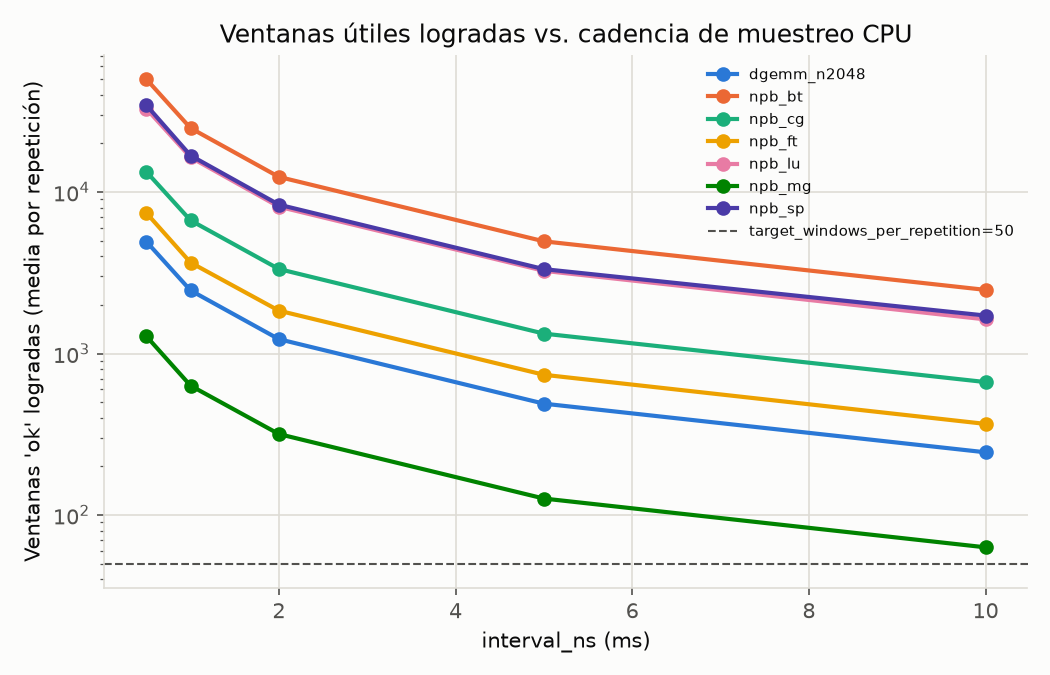
\includegraphics[width=0.85\textwidth]{../plots/interval_ns/windows_ok_vs_interval.png}
\caption{Ventanas \texttt{ok} logradas (media de 3 repeticiones) en función
de la cadencia de muestreo, para los 7 kernels de dataset CPU.}
\label{fig:interval-windows}
\end{figure}

\subsection{Fidelidad del muestreo: el argumento central para 1\,ms}

La Figura~\ref{fig:interval-fidelity} contiene el hallazgo central de este
barrido, pero el promedio simple que la resume oculta una distribución muy
asimétrica -- necesaria de reportar completa para no sobreestimar la
fuerza del argumento. La Tabla~\ref{tab:interval-cv-dist} da la media, la
mediana y el máximo del CV\% del intervalo real (\texttt{sampling\_interval\_cv\_pct}),
sobre las 21 corridas por cadencia (7 kernels $\times$ 3 repeticiones).

\begin{table}[H]
\centering
\caption{Distribución del CV\% del intervalo de muestreo real, por cadencia nominal (21 corridas c/u).}
\label{tab:interval-cv-dist}
\small
\begin{tabular}{@{}lrrr@{}}
\toprule
\textbf{Cadencia} & \textbf{Media} & \textbf{Mediana} & \textbf{Máximo} \\
\midrule
0{,}5\,ms & 1{,}025\,\% & 0{,}154\,\% & 8{,}448\,\% \\
1\,ms     & 0{,}231\,\% & 0{,}098\,\% & 0{,}882\,\% \\
2\,ms     & 0{,}165\,\% & 0{,}155\,\% & 0{,}209\,\% \\
5\,ms     & 0{,}061\,\% & 0{,}055\,\% & 0{,}105\,\% \\
10\,ms    & 0{,}040\,\% & 0{,}038\,\% & 0{,}070\,\% \\
\bottomrule
\end{tabular}
\end{table}

\begin{figure}[H]
\centering
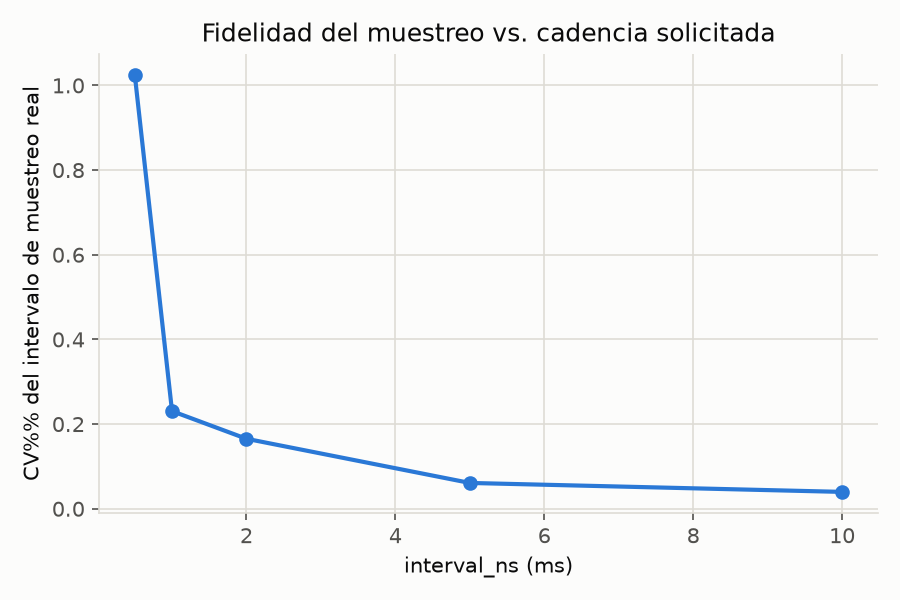
\includegraphics[width=0.75\textwidth]{../plots/interval_ns/sampling_cv_vs_interval.png}
\caption{Fidelidad del muestreo (CV\% del intervalo real vs. el solicitado)
en función de la cadencia. El salto entre 0{,}5\,ms y 1\,ms es la evidencia
central de este barrido.}
\label{fig:interval-fidelity}
\end{figure}

El salto de "más de cuatro veces" en la \textbf{media} (0{,}231\,\%
$\to$ 1{,}025\,\%) está dominado por unas pocas corridas atípicas a
0{,}5\,ms, no por un desplazamiento general de toda la distribución: la
\textbf{mediana} apenas cambia (0{,}098\,\% a 1\,ms vs.\ 0{,}154\,\% a
0{,}5\,ms). Lo que sí cambia de forma clara e inequívoca es el
\textbf{máximo}: 0{,}882\,\% a 1\,ms frente a 8{,}448\,\% a 0{,}5\,ms, casi
diez veces mayor. La lectura correcta no es "la cadencia de 0{,}5\,ms es
en promedio mucho peor", sino que \textbf{0{,}5\,ms es sustancialmente más
vulnerable a eventos ocasionales de interferencia del planificador del
sistema operativo} -- un riesgo de cola, no un sesgo sistemático de toda la
muestra.

Como verificación adicional no reportada en la versión anterior de este
análisis, se recalculó el IPC medio por kernel en cada cadencia respecto a
su propio valor a 1\,ms: la desviación relativa máxima observada, sobre
los 6 kernels CPU con IPC calculable, es de 1{,}93\,\% (\texttt{npb\_sp} a
10\,ms) -- el IPC medido es estable dentro de $\pm$ 2\,\% en todo el rango
0{,}5--10\,ms para todos los kernels probados, así que la cadencia elegida
dentro de ese rango no sesga esta métrica de forma detectable.

\textbf{Conclusión (reformulada)}: 1\,ms es, empíricamente, el primer
punto de la curva en el que el \emph{riesgo de cola} de jitter severo cae
de forma abrupta y donde el IPC medido ya es estable. Es correcto decir
que 1\,ms es un \textbf{valor razonable y conservador, verificado en esta
plataforma}: reduce sustancialmente el riesgo de jitter severo frente a
0{,}5\,ms sin necesitar las ventanas adicionales que 0{,}5\,ms sí ofrece
(aproximadamente el doble, $\sim$20628 vs.\ $\sim$10229 ventanas
\texttt{ok} en promedio sobre los 7 kernels -- corregido respecto a un
valor casi 30 veces menor reportado por un error de conteo en una versión
anterior de este análisis -- una ventaja real, no inexistente, pero
innecesaria frente al objetivo de 50). No es correcto decir que el barrido demuestra que 1\,ms es
"el punto correcto" en un sentido absoluto: no se midió aquí la sobrecarga
propia del instrumento de medición en función de la cadencia, ni la
capacidad de preservar transiciones de carga de duración corta (ambas
quedan como extensiones concretas, no genéricas, de este barrido).


\section{Cadencia de muestreo de GPU (\texttt{gpu\_interval\_ns})}
\label{sec:gpu-interval-ns}

\subsection{Diseño del barrido}

Se corrieron los ocho kernels de dataset GPU del catálogo bajo cinco
cadencias de muestreo NVML (1, 5, 10, 50 y 100\,ms), tres repeticiones cada
una (120 corridas reales). El valor de 100\,ms corresponde al \emph{default}
histórico del instrumento (\texttt{collector.hpp}), vigente en producción
hasta ARC-88 porque \texttt{gpu\_interval\_ns} nunca estuvo declarado como
campo real del manifiesto; 5\,ms es el valor adoptado en ese mismo cambio.

\subsection{El caso que motivó el cambio de producción}

\textbf{Nota sobre una corrección de datos}: la primera versión de este
barrido midió \texttt{rodinia\_heartwall} contra un video sintético que se había
corrompido silenciosamente a 25 cuadros (ver la Sección de hallazgos
colaterales del reporte extendido, ARC-89) -- la corrida fallaba de
inmediato pero seguía marcándose como exitosa, produciendo un patrón de
muestras artificialmente bajo que en un primer momento parecía ser el caso
más ajustado del barrido. Con el video corregido y el kernel re-medido,
\texttt{rodinia\_heartwall} deja de ser un caso límite en absoluto: el caso
real más ajustado es \texttt{rodinia\_backprop}.

La Figura~\ref{fig:gpu-interval} deja ver, con datos nuevos e
independientes de los usados durante la caracterización original, exactamente
el problema que ARC-83/84/86 ya habían diagnosticado con evidencia parcial:
a 100\,ms, \textbf{\texttt{rodinia\_backprop} logra apenas 9{,}0 muestras
NVML útiles en promedio}, apenas por encima del propio
\texttt{target\_windows\_per\_repetition=5}. A 5\,ms (el valor ahora
declarado en el manifiesto de producción), el mismo kernel logra 150{,}3
muestras: un salto de más de un orden de magnitud, no una mejora
incremental. \texttt{rodinia\_heartwall}, ya con datos correctos, se
comporta como el resto del catálogo (1063{,}7 muestras a 5\,ms, 60{,}3 a
100\,ms) -- nunca fue, en realidad, un caso cercano al límite.

\begin{figure}[H]
\centering
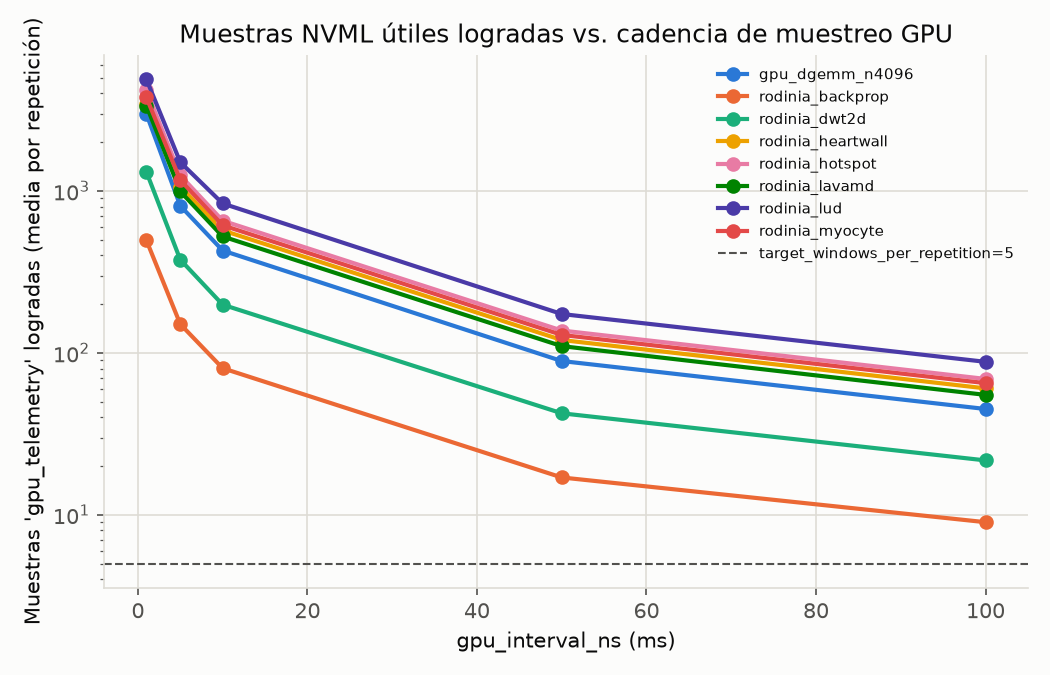
\includegraphics[width=0.85\textwidth]{../plots/gpu_interval_ns/gpu_telemetry_vs_interval.png}
\caption{Muestras NVML útiles logradas (media de 3 repeticiones) en
función de la cadencia de muestreo GPU, para los 8 kernels de dataset GPU
(datos corregidos). \texttt{rodinia\_backprop} es el caso más ajustado del
catálogo.}
\label{fig:gpu-interval}
\end{figure}

Los valores completos de \texttt{rodinia\_backprop} en las cinco cadencias
confirman que el descenso es monótono y suave, no un salto puntual:
150{,}3 muestras a 5\,ms, 80{,}3 a 10\,ms, 17{,}0 a 50\,ms, 9{,}0 a 100\,ms.
Es importante notar que 10\,ms \emph{también} supera el mínimo de 5 con
amplio margen ($16\times$). El valor correcto para describir 100\,ms, dado
el margen de solo $9/5=1{,}8\times$ sobre el mínimo configurado, no es
"insuficiente" en un sentido binario, sino \textbf{frágil y de muy baja
resolución temporal} -- técnicamente pasa el guardarraíl de
\texttt{target\_windows\_per\_repetition}, pero con un margen tan estrecho
que cualquier variación entre repeticiones podría hacerlo fallar. Este
barrido demuestra que 100\,ms es ese caso frágil y que 5\,ms (y también
10\,ms) son viables, pero no aísla a 5\,ms como el único valor correcto
frente a 10\,ms.

\subsection{Contar valores distintos no es lo mismo que contar actualizaciones del sensor}

Un supuesto implícito del argumento anterior es que cada lectura NVML
contada en la Figura~\ref{fig:gpu-interval} es una observación física
nueva. Se verificó esto inspeccionando los valores crudos de
\texttt{gpu\_power\_mw} y \texttt{gpu\_util\_pct} en \texttt{samples.csv}
para \texttt{rodinia\_backprop}, contando \textbf{cambios consecutivos de
valor} como indicador de una actualización real del sensor. Este método
tiene un límite metodológico que debe declararse: si dos actualizaciones
físicas consecutivas del sensor devuelven exactamente el mismo número
(plausible si la potencia se mantiene estable entre dos instantes), el
conteo de "valores distintos" las funde en una sola, subestimando el
número real de actualizaciones -- así que lo medido aquí es una \textbf{tasa
de refresco observada}, una cota inferior de la frecuencia real del
sensor, no una resolución física demostrada de forma directa.

Con esa salvedad, el patrón medido es de todas formas revelador: a 1\,ms
de cadencia (537 lecturas en 0{,}84\,s), solo se observan 7 valores
distintos de potencia, cada uno repetido en promedio 77 veces
consecutivas ($\approx$120\,ms de duración por escalón); a 5\,ms (151
lecturas), 8 valores distintos ($\approx$105\,ms por escalón); a 100\,ms
(9 lecturas), 7 valores distintos -- es decir, a 100\,ms el sondeo ya está
cerca de esta tasa de refresco observada, mientras que a 5\,ms la mayoría
de las "150 muestras" del argumento anterior comparten valor con su
vecina inmediata. \texttt{gpu\_util\_pct} exhibe el mismo patrón (3
valores distintos en 537 lecturas a 1\,ms). Esta periodicidad de
$\sim$105--120\,ms es, hasta donde se pudo verificar, un \textbf{hallazgo
empírico local de este nodo y esta GPU (A100)}: la documentación oficial
de NVML para \texttt{nvmlDeviceGetPowerUsage()} especifica que devuelve
potencia instantánea, pero no garantiza ni documenta una tasa de
actualización de 100--120\,ms -- no debe generalizarse a otro hardware sin
volver a medir.

Esto no invalida la elección de 5\,ms -- el número de lecturas de sondeo
\emph{sí} sigue siendo relevante para otras métricas que podrían variar
más rápido (temperatura, reloj SM, no verificadas aquí) y para reconstruir
la forma temporal de una transición de fase, y sondear más rápido que el
sensor nunca pierde información, solo genera redundancia -- pero sí obliga
a corregir el argumento cuantitativo: el margen "$30\times$" sobre el
objetivo de 5 ventanas cuenta en su mayoría redundancia del muestreo, no
información independiente nueva. La tasa de refresco \emph{observada} en
una corrida típica de \texttt{rodinia\_backprop} (0{,}84\,s) es de
aproximadamente 7--8 escalones distintos, ya cerca del límite de 5 -- un
margen mucho más ajustado que el que sugiere contar lecturas crudas,
aunque el número real de actualizaciones físicas podría ser algo mayor por
la limitación metodológica ya señalada.

\textbf{Conclusión (reformulada)}: la evidencia de este barrido respalda
adoptar 5\,ms como \textbf{valor viable y conservador, verificado en esta
plataforma}, y reclasificar 100\,ms de "insuficiente" a "frágil y de muy
baja resolución temporal, técnicamente por encima del mínimo configurado
pero sin margen real". No queda demostrado que 5\,ms sea el único punto
óptimo frente a 10\,ms (que también es viable y genera menos redundancia
de muestreo), ni que el margen efectivo sobre el mínimo de ventanas sea
tan amplio como sugiere el conteo ingenuo de lecturas -- ese margen real,
aproximado por la tasa de refresco observada y no por las lecturas de
sondeo, es sustancialmente más estrecho. Se recomienda, como extensión
concreta de este hallazgo, medir la duración de cada escalón y su
autocorrelación de forma más rigurosa (no solo contar valores distintos),
y verificar si otras métricas GPU usadas en el proyecto (reloj SM,
temperatura) comparten una tasa de refresco similar.


\section[Repeticiones y ventanas objetivo]{Número de repeticiones (\texttt{repetitions\_per\_combination}) y ventanas objetivo (\texttt{target\_windows\_per\_repetition})}
\label{sec:repetitions}

\subsection{Diseño del barrido}

Se corrieron los 15 kernels de dataset del catálogo (7 CPU, 8 GPU) diez
veces cada uno bajo la cadencia por defecto (150 corridas reales), para
poder calcular, sobre el mismo conjunto de datos, el CV\% de tiempo de
ejecución en función de cuántas de esas diez repeticiones se acumulan
($n=3,4,\ldots,10$) -- sin necesidad de una campaña nueva por cada valor de
$n$. Al procesar los resultados se encontró el mismo error de esta
herramienta de barrido ya descrito en la Sección~\ref{sec:interval-ns}
(\texttt{freq\_khz\_observed=None}); se corrigió de la misma forma,
reprocesando \texttt{samples.csv} sin recolectar datos nuevos.

\subsection{Convergencia de CV\% de tiempo de ejecución}

Las Figuras~\ref{fig:rep-cpu} y~\ref{fig:rep-gpu} muestran la convergencia
por dispositivo. La mayoría de los kernels son estables desde $n=3$: el CV\%
apenas cambia al agregar más repeticiones (\texttt{dgemm\_n2048},
\texttt{npb\_bt}, \texttt{npb\_mg}, \texttt{rodinia\_backprop},
\texttt{rodinia\_heartwall} permanecen por debajo de 0{,}5\,\% en todo el
rango). Dos casos merecen atención:

\begin{itemize}
  \item \textbf{\texttt{rodinia\_lud}} tiene un CV\% estable ($\sim$1{,}3\,\%)
    hasta $n=6$, y salta a 3{,}76\,\% en $n=7$ -- causado por una única
    repetición atípica real (la séptima, 8{,}34\,s frente a un rango normal
    de 9{,}1--9{,}4\,s en las otras nueve, una desviación de $\sim$10\,\%
    respecto a la línea base). Esta es la evidencia más honesta de este
    barrido: con solo tres repeticiones (el mínimo configurado), esta
    anomalía nunca se habría observado, porque el CV\% a $n=3$ (1{,}33\,\%)
    no la refleja en absoluto -- las tres primeras repeticiones no
    incluyen la séptima.
  \item \textbf{\texttt{npb\_ft}} parte de un CV\% relativamente alto a
    $n=3$ (2{,}75\,\%) que decrece de forma monótona hasta 1{,}82\,\% en
    $n=10$ -- consistente con que la variabilidad real del kernel es
    más cercana a 1{,}8--2\,\%, y que la estimación con solo tres
    repeticiones la sobreestima moderadamente por ruido de muestra pequeña,
    no por un problema del kernel o del instrumento.
\end{itemize}

\begin{figure}[H]
\centering
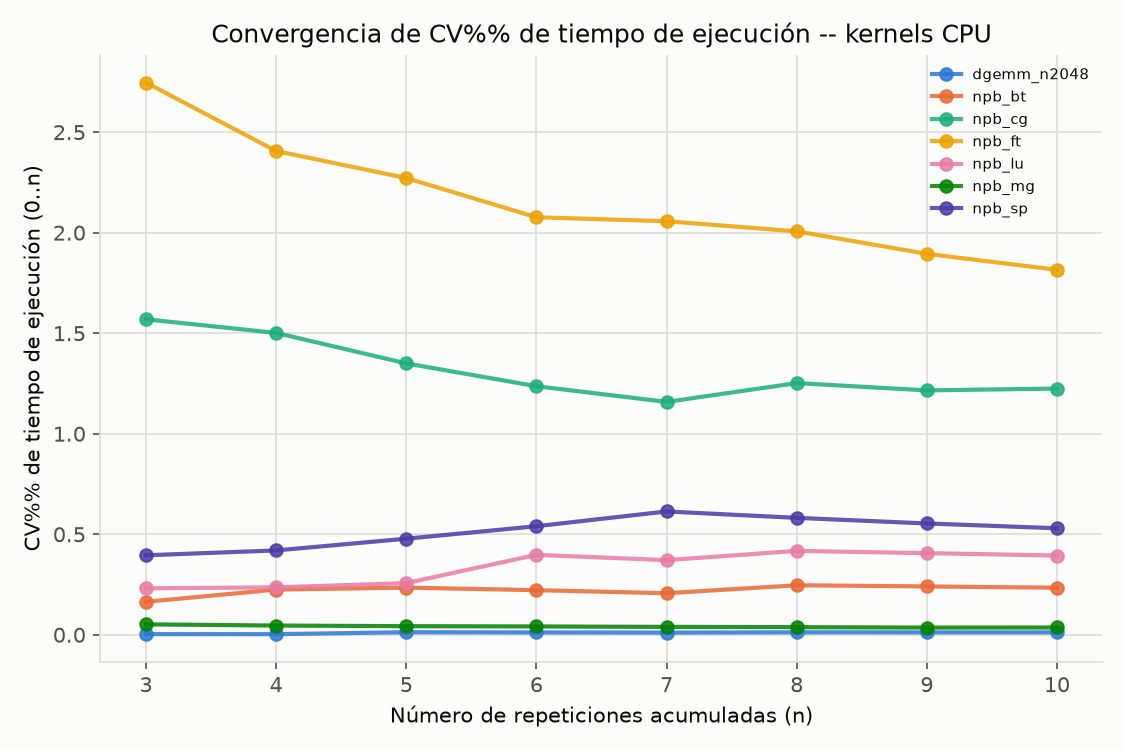
\includegraphics[width=0.85\textwidth]{../plots/repetitions/cv_convergence_vs_repetitions_cpu.png}
\caption{Convergencia de CV\% de tiempo de ejecución vs. repeticiones
acumuladas, kernels CPU.}
\label{fig:rep-cpu}
\end{figure}

\begin{figure}[H]
\centering
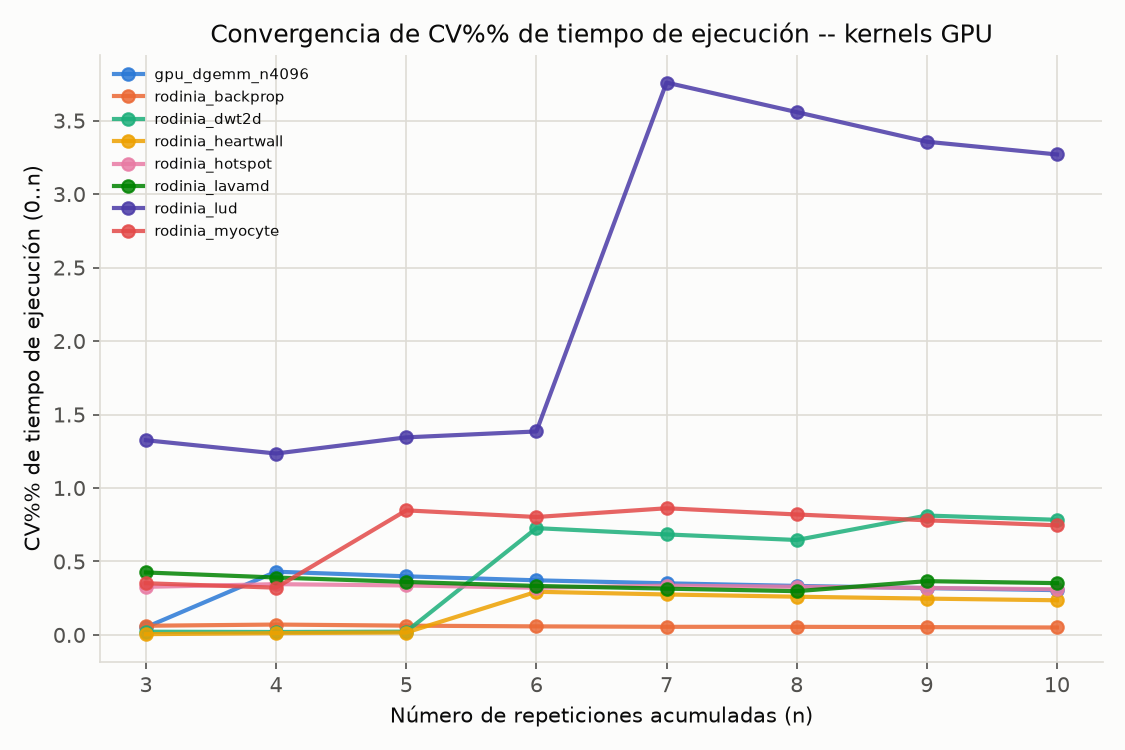
\includegraphics[width=0.85\textwidth]{../plots/repetitions/cv_convergence_vs_repetitions_gpu.png}
\caption{Convergencia de CV\% de tiempo de ejecución vs. repeticiones
acumuladas, kernels GPU. El salto de \texttt{rodinia\_lud} en $n=7$ es una
repetición atípica real, no un artefacto de graficación.}
\label{fig:rep-gpu}
\end{figure}

\subsection{El CV\% de "las primeras tres" depende del orden -- reanálisis combinatorio}

El CV\% a $n=3$ reportado arriba usa siempre las primeras tres de las diez
repeticiones, en el orden fijo en que se ejecutaron. Eso es exactamente el
grupo de tres que una campaña real con \texttt{repetitions\_per\_combination=3}
habría medido -- pero no dice nada sobre qué tan representativo es ese
grupo particular frente a cualquier otro trío posible. Para responder eso,
se recalculó el CV\% de tiempo de ejecución sobre las
$\binom{10}{3}=120$ combinaciones posibles de tres repeticiones de cada
kernel (mismos datos, sin cómputo nuevo), y se compara la muestra de orden
fijo contra la distribución completa (Tabla~\ref{tab:combinatoric-cv3}).

\textbf{Nota metodológica sobre el estimador}: todos los CV\% de esta
sección (y del resto del informe) se calculan con desviación estándar
\emph{poblacional} (\texttt{statistics.pstdev}, denominador $n$), no
muestral (denominador $n-1$). Para $n=3$, la desviación muestral es un
factor $\sqrt{3/2}\approx 1{,}22$ mayor que la poblacional -- es decir,
todos los CV\% a $n=3$ reportados aquí subestiman en $\sim$22\,\% lo que
un cálculo con el estimador insesgado habitual (muestral) reportaría. Esto
no cambia ninguna conclusión cualitativa (qué kernel es más o menos
estable, dónde está la anomalía de \texttt{rodinia\_lud}), pero sí debe
declararse: el margen real de cualquier comparación contra un umbral de
CV\% en este informe es algo más estrecho de lo que las cifras crudas
sugieren.

\begin{table}[H]
\centering
\caption{CV\% de tiempo de ejecución con 3 repeticiones: valor de orden fijo vs. distribución sobre las 120 combinaciones posibles (casos más informativos).}
\label{tab:combinatoric-cv3}
\small
\begin{tabular}{@{}lrrrrr@{}}
\toprule
\textbf{Kernel} & \textbf{orden fijo} & \textbf{mediana} & \textbf{p95} & \textbf{máx} & \textbf{CV\% con n=10} \\
\midrule
\texttt{rodinia\_lud}    & 1{,}32\,\% & 1{,}35\,\% & 5{,}27\,\% & 5{,}49\,\% & 3{,}27\,\% \\
\texttt{npb\_ft}         & 2{,}75\,\% & 1{,}10\,\% & 2{,}51\,\% & 2{,}75\,\% & 1{,}81\,\% \\
\texttt{rodinia\_dwt2d}  & 0{,}02\,\% & 0{,}91\,\% & 0{,}93\,\% & 0{,}93\,\% & 0{,}78\,\% \\
\texttt{rodinia\_myocyte}& 0{,}35\,\% & 0{,}36\,\% & 1{,}21\,\% & 1{,}25\,\% & 0{,}75\,\% \\
\texttt{npb\_cg}         & 1{,}57\,\% & 0{,}91\,\% & 1{,}78\,\% & 1{,}92\,\% & 1{,}23\,\% \\
\bottomrule
\end{tabular}
\end{table}

Dos patrones reales aparecen, y son distintos entre sí:

\begin{itemize}
  \item \textbf{\texttt{rodinia\_lud}}: el trío de orden fijo (1{,}32\,\%) y
    la mediana de los 120 tríos (1{,}35\,\%) coinciden -- la mayoría de los
    tríos posibles \emph{no} incluyen la repetición atípica (rep07). Pero
    el percentil 95 (5{,}27\,\%) y el máximo (5{,}49\,\%) muestran que un
    trío con mala suerte sí la detectaría con un CV\% muy por encima del
    umbral típico de calibración (D03=40\,\% es otro parámetro, no
    comparable directamente, pero un 5\,\% ya es una señal visible en
    cualquier chequeo de estabilidad con umbral de un dígito). Es decir:
    tres repeticiones \emph{pueden} detectar esta anomalía, pero depende
    del azar de cuáles tres se corran -- no es una garantía ni una omisión
    sistemática.
  \item \textbf{\texttt{rodinia\_dwt2d}}: el caso inverso. El trío de orden
    fijo (0{,}02\,\%) es un caso particularmente favorable -- la mediana
    real (0{,}91\,\%) y el CV\% a $n=10$ (0{,}78\,\%) son casi 40 veces
    más altos. Aquí el riesgo no es una anomalía puntual sino que la
    muestra de tres repeticiones normalmente vista subestima la
    variabilidad real del kernel por casi dos órdenes de magnitud respecto
    al trío que efectivamente corrió.
\end{itemize}

\textbf{Conclusión (reformulada tras el reanálisis combinatorio)}: tres
repeticiones constituyen un \textbf{mínimo operativo razonable para la
adquisición de Fase 1} en los kernels alejados de la frontera de
clasificación Roofline, no una demostración de que tres repeticiones
estimen con precisión la variabilidad real de cada kernel ni que
garanticen detectar eventos infrecuentes -- ambas cosas dependen de qué
trío particular se ejecute, como muestra la dispersión completa de
\texttt{rodinia\_lud} y \texttt{rodinia\_dwt2d}. Esta limitación es más
seria para la evaluación de energía y EDP de Fase 4 que para la
adquisición de Fase 1: este barrido caracterizó variabilidad de
\emph{tiempo de ejecución}, no variabilidad energética, y no hay evidencia
todavía de que tres repeticiones sean suficientes para estimar el EDP con
la misma confianza. Para Fase 4 conviene usar más repeticiones o un
criterio adaptativo basado en el ancho del intervalo de confianza
observado, en vez de heredar sin más el mínimo de Fase 1.

\subsection{Suficiencia de \texttt{target\_windows\_per\_repetition}}

Usando las mismas 150 corridas, la Tabla~\ref{tab:target-windows} reporta,
para cada kernel, el mínimo de ventanas útiles logradas en cualquiera de
las diez repeticiones (\texttt{windows\_achieved\_min}) frente al objetivo
configurado (50 para CPU, 5 para GPU). En los 15 kernels del catálogo, el
mínimo observado supera el objetivo por al menos un orden de magnitud
(\texttt{npb\_mg}, el caso más ajustado del lado CPU, con 629 ventanas
mínimas frente a un objetivo de 50; \texttt{rodinia\_backprop}, el más
ajustado del lado GPU, con 140 frente a un objetivo de 5).

\begin{table}[H]
\centering
\caption{Ventanas útiles logradas (media y mínimo sobre 10 repeticiones) vs. objetivo configurado.}
\label{tab:target-windows}
\small
\begin{tabular}{@{}lrrr@{}}
\toprule
\textbf{Kernel} & \textbf{Objetivo} & \textbf{Media} & \textbf{Mínimo} \\
\midrule
\texttt{dgemm\_n2048} & 50 & 2464{,}7 & 2457 \\
\texttt{npb\_bt} & 50 & 24920{,}5 & 24828 \\
\texttt{npb\_cg} & 50 & 6692{,}7 & 6605 \\
\texttt{npb\_ft} & 50 & 3718{,}4 & 3649 \\
\texttt{npb\_lu} & 50 & 16347{,}1 & 16212 \\
\texttt{npb\_mg} & 50 & 637{,}1 & 629 \\
\texttt{npb\_sp} & 50 & 16758{,}7 & 16601 \\
\midrule
\texttt{gpu\_dgemm\_n4096} & 5 & 798{,}2 & 750 \\
\texttt{rodinia\_backprop} & 5 & 148{,}0 & 140 \\
\texttt{rodinia\_dwt2d} & 5 & 375{,}2 & 366 \\
\texttt{rodinia\_heartwall} & 5 & 1064{,}3 & 1058 \\
\texttt{rodinia\_hotspot} & 5 & 1231{,}6 & 1165 \\
\texttt{rodinia\_lavamd} & 5 & 980{,}7 & 922 \\
\texttt{rodinia\_lud} & 5 & 1564{,}2 & 1413 \\
\texttt{rodinia\_myocyte} & 5 & 1152{,}4 & 1113 \\
\bottomrule
\end{tabular}
\end{table}

\textbf{Conclusión (con el alcance correcto del chequeo)}: los datos
demuestran con claridad que \texttt{target\_windows\_per\_repetition}
\textbf{no condiciona el catálogo actual} -- en ningún caso observado
(150 corridas) estuvo cerca de ser la restricción activa, y el margen es
tan amplio (10--500$\times$ el objetivo contando lecturas crudas) que el
valor exacto configurado (50 o 5) no cambia qué corridas se aceptan hoy.
Eso es una afirmación distinta, y más débil, de decir que 50 o 5 son un
\emph{mínimo estadísticamente suficiente}: las ventanas contiguas de un
mismo kernel están correlacionadas entre sí (no son extracciones
independientes de una distribución), y para los kernels GPU, la
Sección~\ref{sec:gpu-interval-ns} muestra que varias "ventanas" NVML
consecutivas pueden compartir el mismo valor de sensor subyacente -- 5
lecturas GPU no equivalen necesariamente a 5 observaciones físicas
distintas. \texttt{target\_windows\_per\_repetition} debe entenderse,
entonces, como un \textbf{guardarraíl de duración mínima de la corrida}
(evita aceptar un kernel que termina casi de inmediato, sin tiempo
suficiente para que el detector de calentamiento y el resto del pipeline
operen con sentido) y no como una prueba de suficiencia estadística de la
muestra resultante. En la práctica, para el catálogo actual, ese
guardarraíl nunca es la restricción activa -- los seis casos ya
documentados con evidencia negativa de calentamiento (ARC-86) son
precisamente ejemplos de kernels cerca del límite en duración total,
aunque no en conteo de ventanas -- pero esto no debe leerse como una
validación de que el dataset resultante tiene suficiencia estadística
para ningún uso posterior (por ejemplo, entrenamiento de un modelo en
Fase 2): esa es una pregunta distinta, que requiere su propio análisis
de partición por corrida/carga, balance de clases y evaluación fuera de
muestra.



\section{Política de \textit{hyperthreading} (\texttt{smt\_policy})}
\label{sec:smt-policy}

A diferencia de F0--F4, la política de \textit{hyperthreading}
(\texttt{smt\_policy}) sí se pudo medir directamente hoy: cambiarla no
requiere el permiso de escritura de frecuencia (P1/P4) que bloquea F0--F4,
porque \texttt{smt\_policy} solo determina qué IDs de CPU se declaran en
\texttt{cores.delegated\_cpus} -- una operación de afinidad
(\texttt{sched\_setaffinity()}) sin privilegios especiales, no una
escritura a \texttt{scaling\_governor} ni a MSRs de frecuencia.

\textbf{Diseño del barrido}: se fijaron los mismos 6 núcleos físicos de
\texttt{paccaA100} (0--5, confirmados vía \texttt{lscpu -e}) y se corrió
\texttt{npb\_cg} --- el kernel de referencia sugerido en el informe
anterior por su sensibilidad conocida a contención de caché --- bajo dos
configuraciones, 5 repeticiones cada una: (1) \texttt{delegated\_cpus=[0..5]},
\texttt{smt\_policy=one\_thread\_per\_physical\_core}, 6 hilos OMP, la
política vigente en producción; (2) \texttt{delegated\_cpus=[0,16,1,17,2,18,
3,19,4,20,5,21]} (ambos hermanos SMT reales de cada uno de los mismos 6
núcleos físicos), \texttt{smt\_policy=all\_threads}, 12 hilos OMP.

\begin{table}[H]
\centering
\caption{IPC medio, MPKI y tasa de fallos LLC, npb\_cg, 6 núcleos físicos fijos (5 repeticiones c/u).}
\label{tab:smt-policy}
\small
\begin{tabular}{@{}lrrrrr@{}}
\toprule
\textbf{Política} & \textbf{Hilos} & \textbf{IPC medio} & \textbf{CV\% IPC} & \textbf{MPKI} & \textbf{Tasa fallos LLC} \\
\midrule
\texttt{one\_thread\_per\_physical\_core} & 6  & 1{,}770 & 0{,}45\,\% & 20{,}80 & 0{,}865 \\
\texttt{all\_threads}                     & 12 & 1{,}055 & 0{,}44\,\% & 20{,}81 & 0{,}865 \\
\bottomrule
\end{tabular}
\end{table}

\begin{figure}[H]
\centering
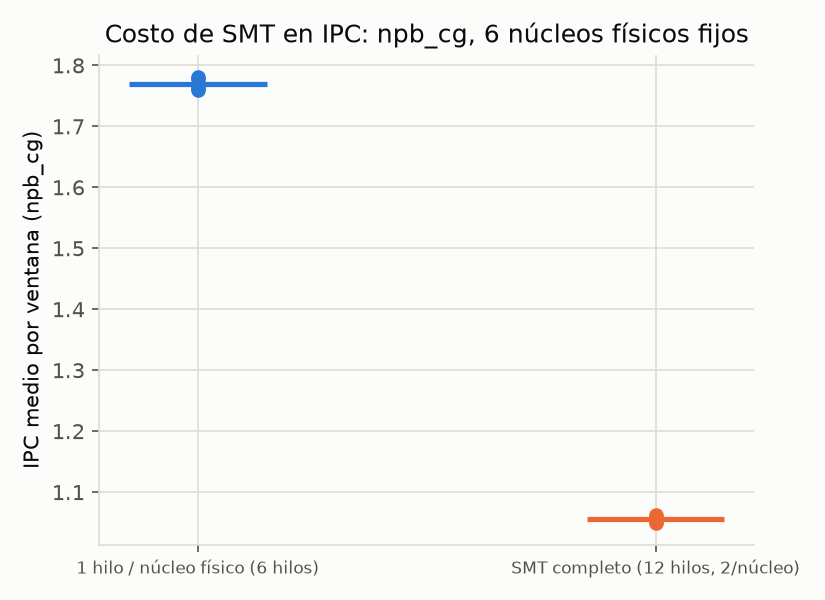
\includegraphics[width=0.75\textwidth]{../plots/smt_policy_ipc.png}
\caption{IPC por ventana, npb\_cg, 5 repeticiones por política (línea horizontal = media).}
\label{fig:smt-policy-ipc}
\end{figure}

\textbf{Resultado}: activar ambos hermanos SMT en los mismos 6 núcleos
físicos reduce el IPC medio de \texttt{npb\_cg} en 40{,}4\,\% (1{,}770 a
1{,}055), con una variabilidad intra-política casi idéntica y despreciable
en ambos casos (CV\%$<$0{,}5\,\% en las dos), es decir, el efecto es
sistemático y no ruido de medición. Notablemente, MPKI y la tasa de fallos
de LLC \textbf{no cambian} entre políticas (20{,}80 vs.\ 20{,}81 MPKI;
0{,}865 en ambas) -- eso descarta que la caída de IPC venga de más tráfico
de caché de último nivel.

\textbf{Límite real de este diseño experimental, que debe declararse}:
esta comparación cambia dos cosas a la vez, no solo la ocupación de SMT --
al pasar de 6 a 12 \texttt{delegated\_cpus}, \texttt{OMP\_NUM\_THREADS}
también pasa de 6 a 12, así que el paralelismo de OpenMP de \texttt{npb\_cg}
cambia junto con la política de SMT. Que MPKI y la tasa de fallos de LLC
se mantengan estables es evidencia compatible con "contención de
\textit{pipeline} entre hermanos SMT" -- el mecanismo que
\texttt{one\_thread\_per\_physical\_core} fue diseñado para evitar -- pero
no la aísla de otras causas posibles del mismo efecto: ancho de banda de
memoria compartido entre los 12 hilos, latencia de sincronización de
OpenMP con el doble de hilos, contención de front-end, o presión sobre las
unidades de carga/almacenamiento. Un diseño que aislara la causa exacta
requeriría mantener \texttt{OMP\_NUM\_THREADS} fijo en 6 y solo cambiar a
qué IDs de CPU se pinan (por ejemplo, 6 hilos sobre 6 núcleos físicos vs.\
6 hilos sobre 3 núcleos físicos con SMT, 2 por núcleo) -- una extensión
concreta no realizada aquí. Lo que sí queda establecido con esta medición,
sin ambigüedad, es que la caída de IPC es real y sistemática bajo SMT
completo, no que su causa exacta sea única y exclusivamente contención de
\textit{pipeline}.

El tiempo total de pared fue, además, \textbf{menor} bajo
\texttt{all\_threads} (5{,}76\,s vs.\ 6{,}82\,s) -- el doble de hilos
completa el trabajo fijo de \texttt{npb\_cg} más rápido pese al IPC por
hilo más bajo. Como el proyecto optimiza EDP (energía $\times$ tiempo), no
tiempo por sí solo, este resultado \textbf{no permite concluir} que
\texttt{one\_thread\_per\_physical\_core} sea la configuración
energéticamente superior -- no se midió energía en este barrido. Su
justificación aquí es distinta y más limitada: aislar la medición de
telemetría/IPC de Fase 1 de un sesgo de contención conocido, no una
afirmación sobre eficiencia energética.

\textbf{Conclusión (con el alcance correcto)}: \texttt{smt\_policy=one\_thread\_per\_physical\_core}
queda confirmado con medición directa como la política que evita un sesgo
sistemático y grande (40{,}4\,\%) en el IPC medido, con evidencia compatible
con -- pero no exclusivamente demostrativa de -- contención de recursos de
\textit{pipeline} entre hermanos SMT como mecanismo. No debe leerse como
una confirmación de que esta política sea la energéticamente óptima para
Fase 4; esa es una pregunta distinta, no respondida aquí.


\section{Sensibilidad del detector de calentamiento}
\label{sec:warmup-sensitivity}

\subsection{Parámetros auditados}

\texttt{scripts/pacca/measure\_warmup.py} determina el intervalo de
calentamiento de cada kernel mediante un umbral de coeficiente de variación
(CV\%) sobre una señal de carga (IPC en CPU, utilización de GPU reportada
por NVML en GPU), con un método de respaldo por detección de puntos de
cambio cuando el umbral de CV no encuentra un punto estable. Cinco
constantes internas de este procedimiento se auditan aquí:
\texttt{CV\_THRESHOLD\_PCT} (umbral de CV, actualmente 5\,\%),
\texttt{MARGIN} (margen de seguridad multiplicativo sobre el punto
detectado, actualmente $\times 1.2$), \texttt{min\_mean\_floor} (piso de
ruido para señales de GPU, actualmente 5{,}0\,\% de utilización),
\texttt{plateau\_ratio} (fracción de la meseta de mayor carga que debe
alcanzar un segmento para aceptarse como fin del calentamiento en el
método de respaldo, actualmente 0{,}8) y los parámetros internos de
segmentación (\texttt{min\_relative\_gain}, \texttt{max\_depth}).

A diferencia de los demás barridos de este informe, este no requirió
cómputo nuevo en \texttt{paccaA100}: se reprocesaron las trazas crudas ya
recolectadas durante la caracterización del catálogo (tres kernels GPU con
transición de carga real -- \texttt{rodinia\_hotspot}, \texttt{rodinia\_heartwall},
\texttt{rodinia\_lavamd} -- y tres kernels CPU con fases conocidas --
\texttt{npb\_bt}, \texttt{npb\_cg}, \texttt{rodinia\_lud}), variando cada
parámetro dentro de un rango razonable mientras los demás se mantienen en
su valor por defecto.

\subsection{Piso de ruido GPU (\texttt{min\_mean\_floor}): justificación por punto de inflexión}

La Figura~\ref{fig:sens-floor} muestra el hallazgo más claro de este
barrido: para los tres kernels GPU con transición de carga real, el
calentamiento detectado es \textbf{0 o casi 0 cuando el piso de ruido está
en 0 o 2\,\%}, y se estabiliza en el valor físicamente correcto (confirmado
contra la traza cruda de potencia en el catálogo, ARC-86) en 5\,\%, 8\,\%
y 12\,\% -- los tres dan el mismo resultado. El rango probado
(0, 2, 5, 8, 12\,\%) tiene un salto de 3 puntos porcentuales entre el
último valor degenerado (2\,\%) y el primer valor estable (5\,\%): esto
demuestra que el punto de inflexión real está \emph{en algún lugar dentro
de ese intervalo (2, 5]\,\%}, y que 5\,\% ya está del lado correcto con
margen (comparte resultado con 8\,\% y 12\,\%, muy por encima del umbral),
pero \textbf{no} que 5\,\% sea, cifra exacta, el punto de inflexión --
eso requeriría un barrido más fino entre 2\,\% y 5\,\% (por ejemplo, cada
0{,}5 puntos) que no se hizo aquí. Lo que sí puede afirmarse sin matices:
por debajo de ese intervalo, el detector cae en el modo de falla original
que motivó introducir este parámetro (una ventana de utilización cercana a
cero se declara ``estable'' por construcción del coeficiente de
variación), y 5\,\% está de forma demostrada e inequívoca del lado
correcto, con margen de sobra hasta 12\,\%.

\begin{figure}[H]
\centering
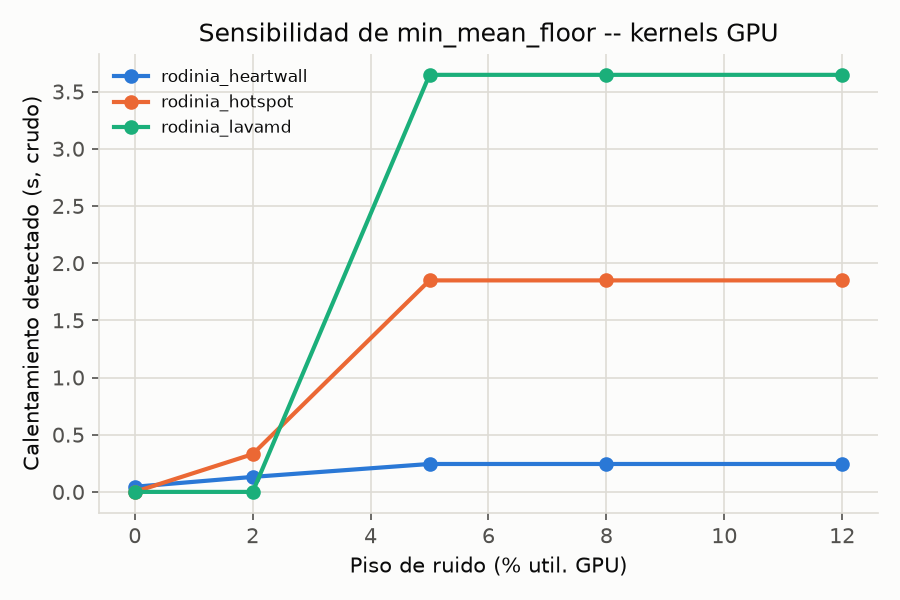
\includegraphics[width=0.85\textwidth]{../plots/warmup_sensitivity/sensitivity_min_mean_floor_gpu.png}
\caption{Calentamiento detectado en función del piso de ruido GPU, para los
tres kernels con transición de carga real. La meseta a partir de 5\,\%
confirma que el valor actual está del lado correcto y con margen del
punto de inflexión (ubicado en algún punto del intervalo (2,5]\,\%, no
resuelto con mayor precisión aquí).}
\label{fig:sens-floor}
\end{figure}

\subsection{Umbral de CV\% (\texttt{CV\_THRESHOLD\_PCT}): robusto en la mayoría de los casos, con una excepción real}

Georges, Buytaert y Eeckhout \citep{Georges2007} recomiendan un umbral de
1--2\,\% para este método; conviene precisar que ese umbral se estableció
para la máquina virtual de Java (variabilidad introducida por JIT y
recolector de basura), un contexto distinto al de un kernel HPC nativo sin
capas de gestión en tiempo de ejecución, así que se cita como antecedente
metodológico del propio método de detección de calentamiento por CV\%, no
como una recomendación directamente transferible al valor numérico usado
aquí. El proyecto usa 5\,\% (heredado del chequeo de estabilidad de
referencia CAL-10, no de la literatura). La
Figura~\ref{fig:sens-cv} muestra el resultado de barrer el umbral entre
1\,\% y 10\,\% sobre los seis kernels:

\begin{itemize}
  \item \texttt{rodinia\_hotspot}, \texttt{rodinia\_heartwall},
    \texttt{rodinia\_lavamd} y \texttt{npb\_bt} son \textbf{completamente
    robustos} en todo el rango 1--10\,\%: el punto detectado no cambia en
    absoluto.
  \item \texttt{npb\_cg} es robusto entre 1\,\% y 8\,\%, pero a 10\,\% la
    detección colapsa a 0\,s (falso positivo) -- evidencia de que el
    umbral no puede subirse indefinidamente sin reintroducir el modo de
    falla, aunque 5\,\% conserva margen de sobra frente a ese límite.
  \item \texttt{rodinia\_lud} es el caso genuinamente sensible: el punto
    detectado se mueve de 0{,}230\,s (8--10\,\%) a 0{,}268\,s (5\,\%) a
    0{,}290\,s (2\,\%), y a 1\,\% el criterio de CV ya no encuentra ningún
    punto y cae al método de respaldo. La variación relativa entre 2\,\% y
    8\,\% es de apenas 0{,}06\,s sobre una corrida de $\sim$12\,s -- no
    altera ninguna conclusión práctica, pero es la evidencia honesta de que
    no todos los kernels son igual de robustos a esta elección.
\end{itemize}

\begin{figure}[H]
\centering
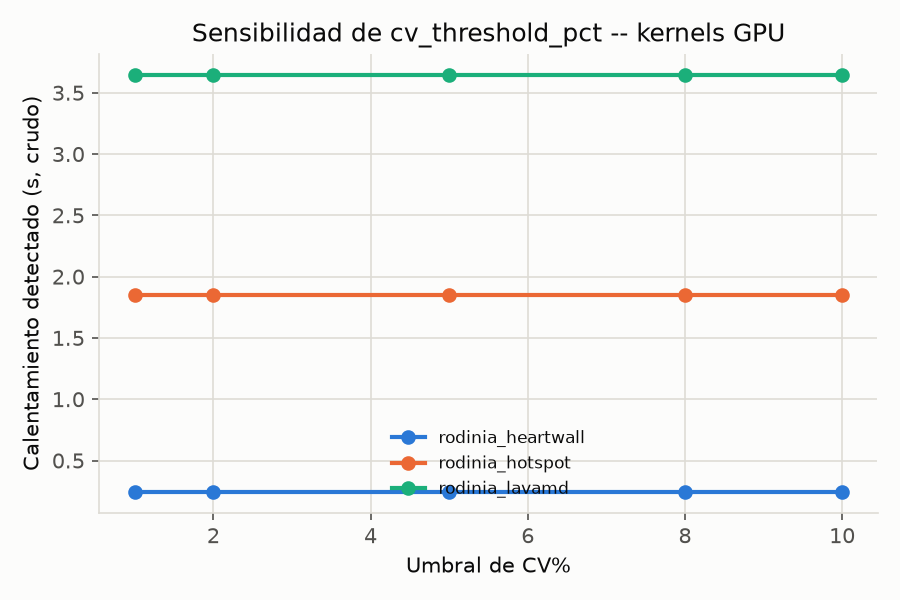
\includegraphics[width=0.85\textwidth]{../plots/warmup_sensitivity/sensitivity_cv_threshold_pct_gpu.png}
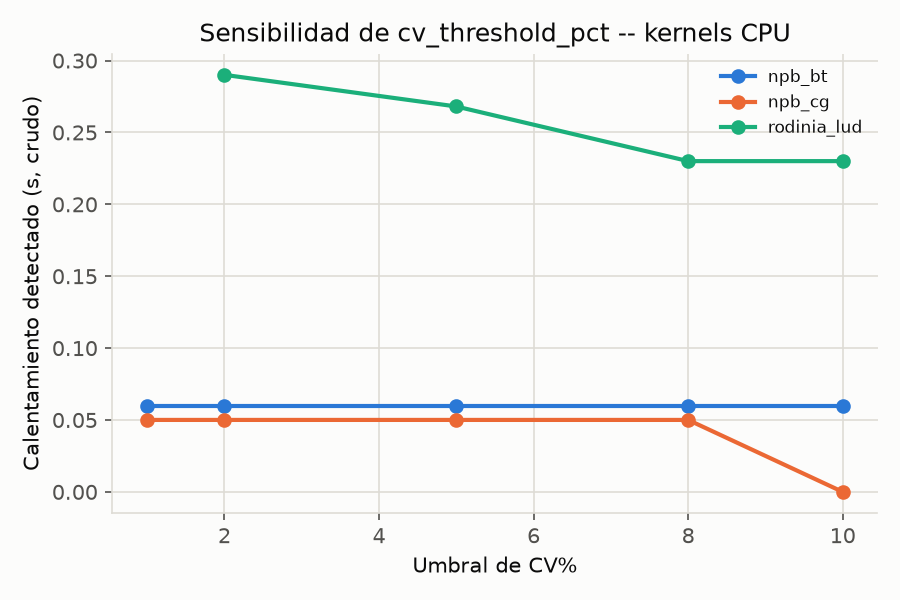
\includegraphics[width=0.85\textwidth]{../plots/warmup_sensitivity/sensitivity_cv_threshold_pct_cpu.png}
\caption{Calentamiento detectado en función del umbral de CV\%, kernels GPU
(arriba) y CPU (abajo). La mayoría de las líneas son planas (robustas); la
de \texttt{rodinia\_lud} tiene pendiente real, y la de \texttt{npb\_cg} cae
a cero en el extremo derecho.}
\label{fig:sens-cv}
\end{figure}

\textbf{Conclusión}: el umbral de 5\,\% queda confirmado como una elección
segura -- ni tan bajo como para perder detección en \texttt{rodinia\_lud},
ni tan alto como para caer en el falso positivo de \texttt{npb\_cg} a
10\,\% -- pero su origen (``prestado'' de CAL-10, no derivado
independientemente) sigue sin una justificación de primer principio más
allá de esta verificación empírica de robustez.

\subsection{Margen de seguridad (\texttt{MARGIN})}

El margen es, por construcción, una función lineal del punto crudo
detectado ($t_{\text{propuesto}} = t_{\text{crudo}} \times \text{margen}$),
así que no hay una relación no trivial que descubrir aquí -- la
Figura~\ref{fig:sens-margin} simplemente cuantifica cuántos segundos
representa cada opción de margen para los kernels reales. Para
\texttt{rodinia\_lavamd}, el kernel con mayor calentamiento absoluto, la
diferencia entre no aplicar margen ($\times 1.0$) y el valor actual
($\times 1.2$) es de 0{,}73\,s; para \texttt{npb\_cg}, de apenas 0{,}01\,s.
No se encontró evidencia de que $\times 1.2$ sea insuficiente o excesivo en
ningún caso real -- la elección permanece una decisión de ingeniería
razonable sin una derivación estadística propia (por ejemplo, a partir de
la varianza del punto detectado entre repeticiones), que queda como
mejora futura.

\begin{figure}[H]
\centering
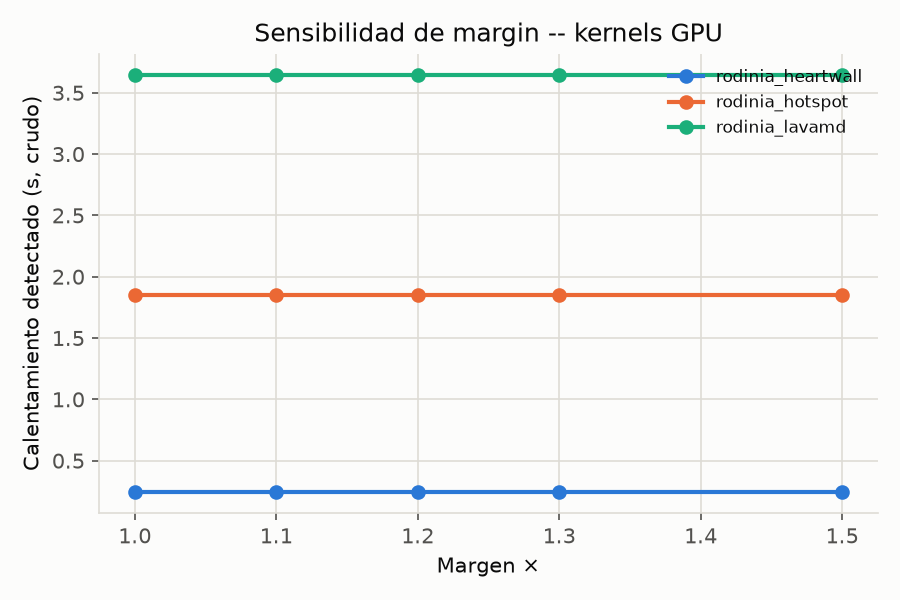
\includegraphics[width=0.85\textwidth]{../plots/warmup_sensitivity/sensitivity_margin_gpu.png}
\caption{Calentamiento propuesto (crudo × margen) en función del margen de
seguridad, kernels GPU.}
\label{fig:sens-margin}
\end{figure}

\subsection{Fracción de meseta (\texttt{plateau\_ratio})}

Ninguno de los seis kernels de esta muestra activó el método de respaldo
por punto de cambio con sus parámetros por defecto (todos se resolvieron
por el umbral de CV), así que este barrido no pudo ejercitar
\texttt{plateau\_ratio} con datos reales de este proyecto -- las líneas son
planas en el rango 0{,}6--0{,}9 simplemente porque el método de respaldo
nunca se invocó. La justificación de 0{,}8 sigue siendo, por tanto, la
descrita en ARC-86 (corrige un modo de falla real observado en
\texttt{rodinia\_hotspot} durante su caracterización), no una verificada
por barrido de sensibilidad en este documento. \textbf{Pendiente}: repetir
este barrido específicamente sobre un kernel que sí caiga en el método de
respaldo (por ejemplo, forzando \texttt{CV\_THRESHOLD\_PCT} a un valor muy
bajo para inducir el respaldo de forma controlada) antes de considerar este
parámetro completamente verificado.


\section{Convergencia del número de lanzamientos perfilados con \texttt{ncu}}
\label{sec:ncu-convergence}

\subsection{Diseño del barrido}

Se perfilaron los siete kernels de dataset GPU (excluyendo
\texttt{gpu\_dgemm\_n4096}, calibrado contra una referencia de cuBLAS por
razones ya documentadas en el catálogo) con \texttt{ncu} bajo tres valores
de \texttt{--launch-count} (5, 20, 50), midiendo el FLOP/byte estimado en
cada caso. Al procesar los resultados se encontró y corrigió un error real
en el script de este barrido (no del instrumento de producción): la
reconstrucción del nombre de la métrica de FMA/suma/multiplicación para
precisión simple omitía el prefijo \texttt{f} (\texttt{..\_fma\_pred\_on}
en vez de \texttt{..\_ffma\_pred\_on}), lo que hacía que los seis kernels
FP32 del barrido reportaran FLOP/byte=0. Los datos crudos de \texttt{ncu} ya
estaban en disco, así que se corrigió re-parseando sin re-perfilar. Un
segundo problema, de datos y no de análisis, afectó a
\texttt{rodinia\_heartwall}: ver la Sección de hallazgos colaterales
(video sintético truncado) -- se resolvió re-generando el video y
re-perfilando ese kernel específicamente.

\subsection{Resultados}

La Figura~\ref{fig:ncu-convergence} y la Tabla~\ref{tab:ncu-convergence}
muestran el FLOP/byte estimado en función del número de lanzamientos
perfilados, junto con el número real de lanzamientos alcanzado (columna
$n$, limitado por cuántas veces el kernel realmente invoca su función
principal -- pedir más lanzamientos de los que el programa ejecuta no
produce más datos).

\begin{table}[H]
\centering
\caption{Convergencia de FLOP/byte vs. número de lanzamientos solicitados a \texttt{ncu}.}
\label{tab:ncu-convergence}
\small
\begin{tabular}{@{}lrrrr@{}}
\toprule
\textbf{Kernel} & \textbf{$n$ real (máx. 3 puntos)} & \textbf{OI a 5} & \textbf{OI a 20/10} & \textbf{OI a 50} \\
\midrule
\texttt{rodinia\_backprop} & 2 (fijo) & 0{,}07987 & 0{,}07987 & 0{,}07986 \\
\texttt{rodinia\_lavamd} & 1 (fijo) & 708{,}49 & 708{,}30 & 708{,}35 \\
\texttt{rodinia\_dwt2d} & 5 / 10 / 10 & 2{,}1762 & 2{,}1762 & 2{,}1741 \\
\texttt{rodinia\_hotspot} & 5 / 20 / 50 & 5{,}0232 & 5{,}0206 & 5{,}0200 \\
\texttt{rodinia\_heartwall} & 5 / 20 / 50 & 35{,}300 & 35{,}297 & 35{,}350 \\
\texttt{rodinia\_myocyte} & 5 / 20 / 50 & 0{,}01704 & 0{,}01692 & 0{,}01704 \\
\texttt{rodinia\_lud} & 5 / 20 / 50 & \textbf{7{,}492} & \textbf{7{,}584} & \textbf{7{,}668} \\
\bottomrule
\end{tabular}
\end{table}

\begin{figure}[H]
\centering
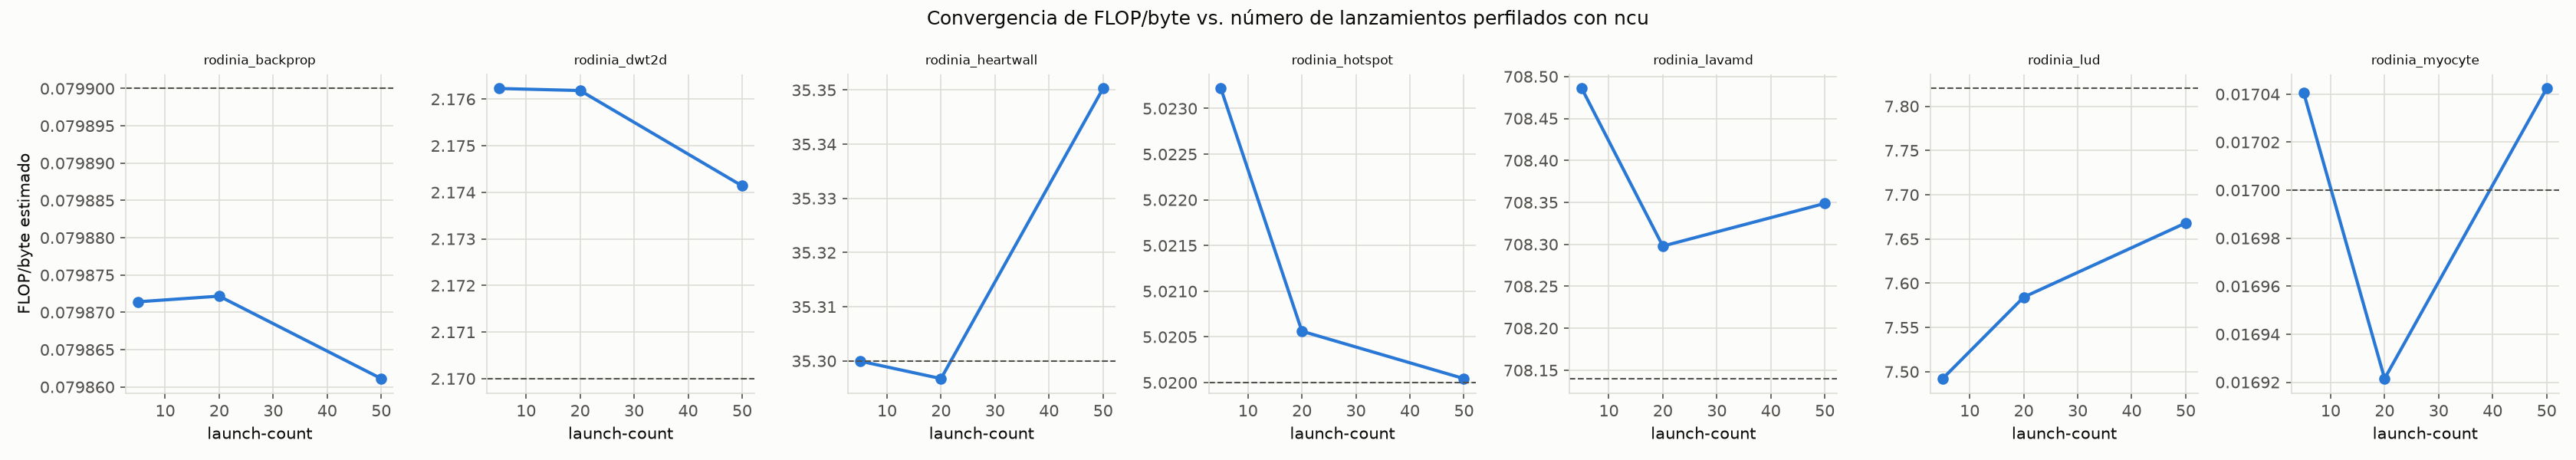
\includegraphics[width=\textwidth]{../plots/ncu_launch_count/ncu_convergence.png}
\caption{FLOP/byte estimado vs. lanzamientos solicitados, siete kernels de
dataset GPU. La línea punteada marca el valor declarado en el catálogo.}
\label{fig:ncu-convergence}
\end{figure}

Seis de los siete kernels no dejan nada que barrer de forma significativa:
\texttt{rodinia\_backprop} y \texttt{rodinia\_lavamd} solo tienen 2 y 1
lanzamiento real respectivamente (sin importar cuántos se soliciten, ya
está el dato completo desde el primer punto); \texttt{rodinia\_dwt2d} se
satura en 10 lanzamientos reales; y \texttt{rodinia\_hotspot},
\texttt{rodinia\_heartwall} y \texttt{rodinia\_myocyte} sí tienen
lanzamientos de sobra pero su FLOP/byte ya es estable dentro de
$\pm$ 0{,}2\,\% desde 5 lanzamientos.

\textbf{\texttt{rodinia\_lud} es la única excepción real}: con lanzamientos
de sobra disponibles, el FLOP/byte estimado sube de forma monótona y no
plateada entre 5 y 50 lanzamientos (7{,}49 $\to$ 7{,}58 $\to$ 7{,}67, una
variación de +2{,}3\,\% sin señal clara de haber convergido en el
extremo superior del rango probado). Esto es significativo precisamente
porque \texttt{rodinia\_lud} es el único kernel del catálogo etiquetado
``intermedio'': su intensidad operacional declarada (7{,}82 FLOP/byte,
ARC-80) queda apenas un 7{,}4\,\% por encima del \emph{ridge} FP32
vainilla medido en este mismo nodo con el probe propio del proyecto
($\approx$7{,}28 FLOP/byte, ARC-76 -- corrección respecto a un valor de
7{,}98 usado en una versión anterior de este análisis, que no correspondía
a ninguna medición del catálogo). Con ese ridge correcto, los tres puntos
de este barrido (7{,}49 a 7{,}67) ya están por \emph{encima} del ridge
desde el primer punto (5 lanzamientos) -- la clasificación
\texttt{compute\_bound} no cambia en el rango medido, pero el margen sobre
el ridge sí cambia de forma sustancial según cuántos lanzamientos se usen
(de 2{,}9\,\% de margen a 5 lanzamientos hasta 4{,}9\,\% a 50), lo cual
importa precisamente porque el caso es borderline por diseño (menos del
8\,\% de margen incluso en el valor ya declarado). Con solo estos tres
puntos, lo único que puede afirmarse es que 50 lanzamientos son
insuficientes para estabilizar ese margen -- no que 200 (el valor ya
declarado en el catálogo, ARC-80) sean el número correcto; extrapolar esa
suficiencia sin medirla sería precisamente el tipo de afirmación
sobredimensionada que este informe busca evitar.

\subsection{Extensión dirigida: cerrando la convergencia de \texttt{rodinia\_lud}}

Se perfilaron tres puntos adicionales para este kernel específicamente
(100, 150 y 200 lanzamientos, 3 corridas de \texttt{ncu} de costo bajo),
aplicando un criterio de convergencia declarado \textbf{antes} de ver el
resultado: convergencia = cambio relativo menor al 1\,\% entre cada par
consecutivo de puntos.

\begin{table}[H]
\centering
\caption{Convergencia extendida de \texttt{rodinia\_lud} (criterio: $\Delta < 1$\,\% pre-declarado).}
\label{tab:lud-convergence-extended}
\small
\begin{tabular}{@{}lrr@{}}
\toprule
\textbf{Lanzamientos} & \textbf{FLOP/byte} & \textbf{Cambio relativo vs. punto anterior} \\
\midrule
5   & 7{,}4922 & -- \\
20  & 7{,}5842 & 1{,}23\,\% \\
50  & 7{,}6680 & 1{,}11\,\% \\
100 & 7{,}7737 & 1{,}38\,\% \\
150 & 7{,}8162 & \textbf{0{,}55\,\%} (converge) \\
200 & 7{,}8240 & 0{,}10\,\% \\
\bottomrule
\end{tabular}
\end{table}

\begin{figure}[H]
\centering
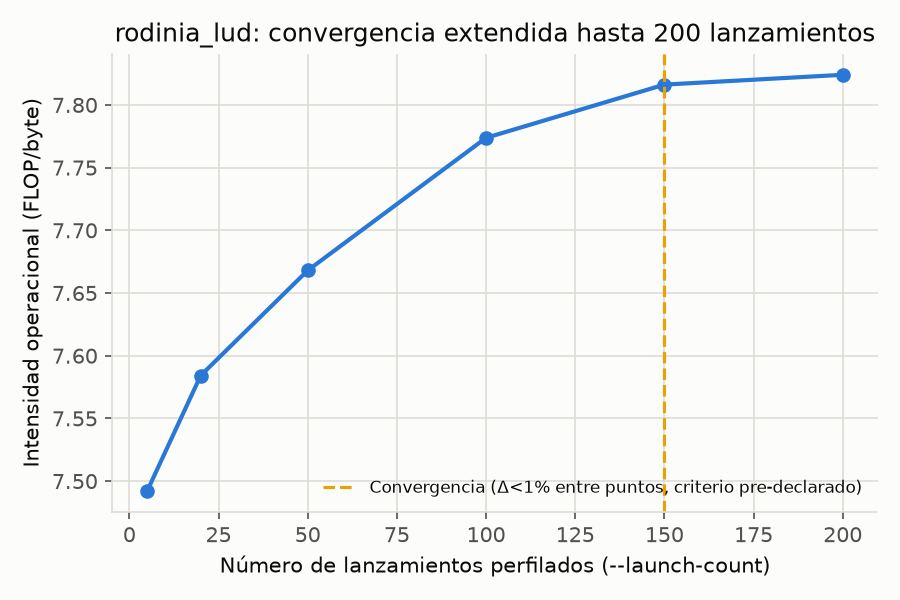
\includegraphics[width=0.75\textwidth]{../plots/lud_ncu_convergence_extended.png}
\caption{Convergencia extendida de \texttt{rodinia\_lud} hasta 200 lanzamientos.}
\label{fig:lud-convergence-extended}
\end{figure}

Con el criterio pre-declarado, la convergencia se alcanza en
\textbf{launch-count=150} (cambio de 0{,}55\,\% respecto al punto
anterior, y de solo 0{,}10\,\% entre 150 y 200). El valor de 200 usado en
el catálogo (ARC-80) queda ahora \textbf{confirmado con medición directa,
no solo con evidencia indirecta de no-convergencia a 50}: 200 lanzamientos
están efectivamente por encima del punto de convergencia real (150), con
un margen razonable, no arbitrariamente por encima de él.

\textbf{Conclusión}: no existe un número de lanzamientos único
correcto para todo el catálogo -- el número real de lanzamientos que cada
kernel ejecuta varía en más de dos órdenes de magnitud (de 1 a cientos), y
la velocidad de convergencia del FLOP/byte estimado varía igual de fuerte.
La práctica correcta, confirmada por este barrido, es perfilar con
suficientes lanzamientos para observar la meseta de convergencia
\emph{de cada kernel individualmente}, aplicando un criterio de
convergencia declarado de antemano -- para los seis kernels estables desde
5 lanzamientos, la evidencia ya alcanza para cerrar el parámetro; para
\texttt{rodinia\_lud}, el caso más exigente, la extensión a 200
lanzamientos cierra el parámetro con el mismo estándar de evidencia, en
vez de con una extrapolación razonable pero no medida.


\section{Distribución empírica de la calibración Roofline}
\label{sec:calibration-distribution}

\subsection{Diseño del barrido}

Se corrieron diez repeticiones independientes de cada uno de los cinco
kernels de calibración del catálogo (\texttt{stream\_official},
\texttt{ert\_probe} para CPU; \texttt{gpu\_stream\_bw},
\texttt{gpu\_ert\_probe\_fp32}, \texttt{gpu\_ert\_probe\_fp64} para GPU),
extrayendo el valor reportado por cada una directamente de su salida
estándar -- sin usar la orquestación completa de calibración
(\texttt{run\_calibration}/\texttt{run\_gpu\_calibration}), que normalmente
solo calibra una vez por campaña.

\subsection{Resultados}

La Figura~\ref{fig:calibration-dist} y la Tabla~\ref{tab:calibration-dist}
muestran la dispersión real de diez mediciones independientes de cada
referencia de calibración.

\begin{table}[H]
\centering
\caption{Dispersión de 10 calibraciones independientes.}
\label{tab:calibration-dist}
\begin{tabular}{@{}lrr@{}}
\toprule
\textbf{Kernel de calibración} & \textbf{CV\% (10 repeticiones)} & \textbf{Desviación vs. referencia declarada} \\
\midrule
\texttt{stream\_official} (BW, CPU) & 0{,}593\,\% & 0{,}10\,\% \\
\texttt{ert\_probe} (FLOPs, CPU) & 0{,}127\,\% & 0{,}23\,\% \\
\texttt{gpu\_stream\_bw} (BW, GPU) & 0{,}628\,\% & sin referencia declarada \\
\texttt{gpu\_ert\_probe\_fp32} (FLOPs, GPU) & 0{,}0012\,\% & sin referencia declarada \\
\texttt{gpu\_ert\_probe\_fp64} (FLOPs, GPU) & 0{,}000016\,\% & sin referencia declarada \\
\bottomrule
\end{tabular}
\end{table}

\begin{figure}[H]
\centering
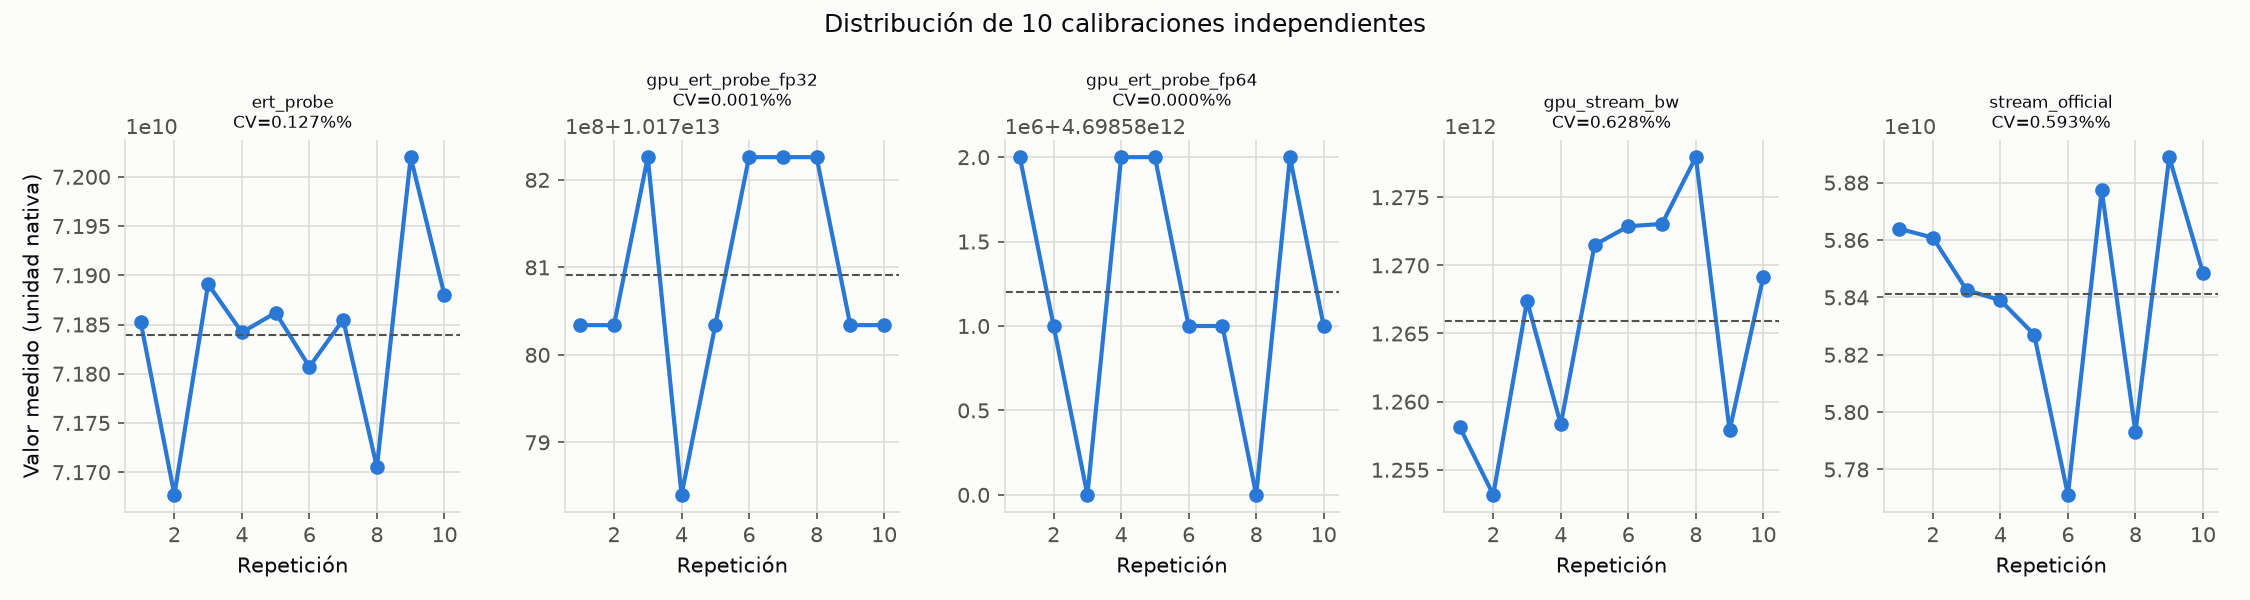
\includegraphics[width=\textwidth]{../plots/calibration_repeats/calibration_distribution.png}
\caption{Diez calibraciones independientes por kernel de referencia. La
línea punteada marca la media. Nótese la escala de cada panel: la
dispersión visual parece grande, pero el eje vertical cubre una fracción
mínima del valor absoluto en todos los casos.}
\label{fig:calibration-dist}
\end{figure}

Los probes de FLOPs de GPU (\texttt{gpu\_ert\_probe\_fp32/fp64}) muestran
una estabilidad extraordinaria (CV\% $<$0{,}002\,\%, y para FP64
0{,}000016\,\% -- esencialmente determinista) -- consistente con el
hallazgo ya documentado en el proyecto (ARC-77) de que la GPU no varía su
reloj bajo carga en este nodo: sin ninguna variabilidad de \textit{boost}
que introducir, el pico de cómputo medido es prácticamente determinista de
una corrida a otra. El ancho de banda (CPU y GPU) y el pico de FLOPs de CPU
muestran algo más de dispersión ($\sim$0{,}1--0{,}6\,\%), coherente con la
variabilidad normal de acceso a memoria compartida del sistema.

Es importante no sobreinterpretar lo que esta baja dispersión demuestra:
que el ruido normal esté en 0{,}1--0{,}6\,\% no dice nada sobre si 40\,\%
es un valor mejor que 10\,\%, 20\,\% o 30\,\% -- ninguno de esos valores
alternativos se comparó aquí. Lo que sí demuestra, y es la única
afirmación que este barrido respalda, es dónde está el ruido de fondo
real frente al cual cualquiera de esas tolerancias tendría que operar.

\textbf{Conclusión sobre \texttt{D03\_TOLERANCE\_FRACTION} (40\,\%, CPU)
-- \emph{guardarraíl conservador confirmado, no tolerancia derivada
estadísticamente}}: esta medición, independiente de la ya reportada en el
reporte anterior (una única calibración de referencia), confirma con diez
repeticiones que la desviación real de la calibración de CPU frente a su
valor de referencia (0{,}10\,\% y 0{,}23\,\%) está casi tres órdenes de
magnitud por debajo del 40\,\% configurado. Esto confirma que el 40\,\%
nunca se ha acercado a su límite en la práctica y que sigue funcionando
como red de seguridad contra errores groseros de configuración (el caso
histórico que la motivó, ARC-55, fue una discrepancia de más de
5$\times$) -- pero no confirma que 40\,\% sea el valor óptimo ni que esté
derivado del ruido medido; es, y debe reportarse como, un margen de
seguridad amplio y deliberadamente conservador, no una tolerancia
estadística ajustada al ruido real.

\textbf{Conclusión sobre la tolerancia cruzada de GPU (5\,\%, sin
datasheet) -- \emph{parcialmente justificada, pendiente de DVFS real}}:
esta medición establece una cota inferior útil -- el ruido de medición
puro de los probes de GPU (0{,}0004--0{,}63\,\%) es tan pequeño que, si una
futura calibración a un nivel de frecuencia distinto de REF mostrara una
diferencia cercana al 5\,\% de tolerancia, esa diferencia casi con toda
seguridad reflejaría un cambio real de frecuencia y no ruido de medición.
Pero esto es evidencia de que el 5\,\% tiene margen frente al ruido de
fondo, no evidencia de que el chequeo efectivamente detecte una aplicación
fallida de frecuencia cuando ocurra: esa verificación end-to-end (aplicar
un nivel de frecuencia real distinto de REF y confirmar que la calibración
cruzada lo detecta) sigue sin poder hacerse hasta que llegue el permiso
P4, y esta tolerancia debe seguir clasificada como parcial, no confirmada,
mientras eso no se verifique.


\section{Parámetros justificados por estado del arte, sin barrido dedicado}
\label{sec:literatura}

Los tres parámetros de esta sección no quedan sin cerrar por alcance o
descuido: cada uno tiene un veredicto explícito y una razón concreta por
la que la medición directa no es la vía adecuada hoy -- un permiso externo
pendiente en un caso, una decisión ética deliberada de no interferir con
infraestructura compartida en otro, y una dependencia real de resultados
que todavía no existen (Fase 4) en el tercero. Ninguno queda como
``trabajo futuro'' genérico: cada uno indica la condición exacta que, de
cumplirse, permitiría cerrarlo con medición.

\subsection{Niveles de frecuencia previstos (F0--F4)}

Los manifiestos de producción declaran cinco niveles fijos equiespaciados
(100\,\%, 75\,\%, 50\,\%, 25\,\% y 0\,\% del rango real de frecuencia
detectado en el nodo) además del nivel de referencia (gobernador nativo).
Esta elección no puede verificarse empíricamente hoy: requiere el permiso
de escritura de frecuencia (P1 para CPU, P4 para GPU), que sigue sin
llegar a la fecha de este informe. Tampoco se encontró en la literatura ya
revisada una recomendación explícita sobre cuántos puntos son suficientes
para caracterizar la curva DVFS de una carga: Guerreiro et al.
\citep{Guerreiro2019} infieren el resto del espacio de frecuencias a partir
de una única frecuencia base, sin barrer puntos uniformes; Ali et al.
\citep{Ali2023} parten igualmente de una configuración base y extrapolan de
forma analítica el resto del espacio, en vez de medir en un conjunto fijo
de puntos como aquí. La elección de cinco puntos equiespaciados es
razonable como decisión de diseño (visibiliza la forma de la curva sin
disparar el tamaño de la matriz experimental), pero no está anclada a un
estudio específico. Queda como pendiente explícito: en cuanto lleguen los
permisos, correr primero un reconocimiento con más puntos (por ejemplo,
nueve, cada 12{,}5\,\%) sobre dos o tres kernels representativos para
verificar si cinco puntos ya capturan la forma real de la curva.

\subsection{Umbral de carga externa (E08) y rango de temperatura (E02)}

\textbf{Corrección importante respecto a una versión anterior de este
análisis, y hallazgo más serio que una simple falta de barrido}: no es
solo que E08 y E02 se excluyan deliberadamente de prueba de estrés por
razones éticas -- una revisión del código de \texttt{preflight.py} y
\texttt{campaign.py} encontró que \textbf{ninguno de los dos chequeos se
ejecuta hoy en ninguna campaña real}. \texttt{run\_campaign\_preflight}
(el preflight que sí se invoca en producción) no incluye ni E02 ni E08;
ambos viven en \texttt{run\_reduced\_preflight}, una función con pruebas
unitarias propias pero que \texttt{campaign.py} nunca llama. Y aunque se
llamara, \texttt{Manifest} no declara el campo
\texttt{package\_temperature\_c} que \texttt{check\_temperature} necesita
-- con ese campo ausente (\texttt{None}), el chequeo aprueba de forma no
bloqueante con el mensaje ``no hay sensor disponible'', nunca bloquea
nada. El mismo tipo de hallazgo aplica al preflight de GPU (G01--G03): el
manifiesto de referencia GPU declara \texttt{gpu.enabled: false}, así que
esos chequeos tampoco corren hoy, y ni siquiera se les pasa un inspector
NVML desde \texttt{cli.py}. Este hallazgo se documenta con el mismo
detalle en la Sección~\ref{sec:metodologia} y en el balance final
(Sección~\ref{sec:balance}); aquí se completa con la justificación
teórica de cada umbral, ahora explícitamente como un umbral \emph{sin
mecanismo de verificación activo}, no como un umbral verificado pero sin
barrido de estrés.

E08 (carga externa normalizada $\leq 1{,}0$) se apoya en la convención
estándar de "nodo no saturado" en HPC, pero merece una precisión: el
propio \texttt{/proc/loadavg} cuenta procesos ejecutables o en espera de
E/S a nivel de \emph{todo el sistema}, no solo los de los núcleos
delegados a la corrida -- dividir esa cifra global entre 6 núcleos
delegados no aísla, por sí solo, si la contaminación ocurre específicamente
sobre esos 6 núcleos o en otra parte del nodo (irrelevante para la corrida
si el nodo tiene núcleos libres en otro socket). El umbral sigue siendo una
señal razonable de saturación general del nodo, pero no un chequeo preciso
de aislamiento por núcleo -- y, de cualquier forma, hoy no se ejecuta en
ninguna corrida real por el hallazgo anterior.

E02 (temperatura de paquete en $[0,90]\,^{\circ}\text{C}$) queda
\textbf{solo parcialmente} justificado por ficha técnica, no confirmado:
la hoja de especificaciones de Intel ARK para el SKU exacto del nodo (Xeon
Gold 5315Y, ARK 215286) documenta una temperatura de caja máxima
($T_{\text{case}}$) de 81\,$^{\circ}$C, no
90\,$^{\circ}$C.\footnote{\url{https://www.intel.com/content/www/us/en/products/sku/215286/}}
La temperatura de unión máxima ($T_j$máx, un límite distinto y típicamente
más alto que $T_{\text{case}}$) no tiene, hasta donde se pudo verificar en
esta revisión, una cifra pública específica para este SKU en ARK -- una
versión anterior de este análisis citaba un rango de 100--110\,$^{\circ}$C
sin fuente oficial que lo respaldara para este procesador en particular, y
se retira aquí por no estar verificado, en vez de mantenerlo sin cita. Lo
que sí queda establecido con fuente verificable es que $T_{\text{case}}$
(81\,$^{\circ}$C) es menor que el umbral configurado (90\,$^{\circ}$C),
así que el margen de seguridad no puede compararse directamente contra
$T_{\text{case}}$ sin aclarar que son magnitudes distintas: ninguna
corresponde exactamente a lo que \texttt{coretemp} reportaría si el sensor
estuviera conectado -- \texttt{coretemp} entrega un DTS (\textit{Digital
Thermal Sensor}) relativo a $T_j$máx, no una lectura directa de
$T_{\text{case}}$; y RAPL, aunque está habilitado en este nodo, mide
energía consumida, no temperatura -- ninguno de los dos provee hoy el dato
que \texttt{package\_temperature\_c} necesitaría. Diseñar E02 comparando
directamente una futura lectura DTS de \texttt{coretemp} contra
$T_{\text{case}}$ sería, por esta razón, metodológicamente incorrecto; el
chequeo, si se activa, debería compararse contra un límite expresado en
los mismos términos que el sensor real (DTS relativo a $T_j$máx). Así que
90\,$^{\circ}$C no puede describirse como "el umbral típico verificado", y
merece una precisión más incómoda que la de una versión anterior de este
análisis: 90\,$^{\circ}$C está \emph{por encima}, no por debajo, de la
única cifra con fuente oficial verificada para este SKU
($T_{\text{case}}=81\,^{\circ}\text{C}$). Que 90\,$^{\circ}$C sea o no un
margen conservador depende enteramente de $T_j$máx (típicamente mayor que
$T_{\text{case}}$ en procesadores Intel modernos, pero sin cifra pública
verificada para este SKU específico) -- una afirmación que no se puede
confirmar ni descartar con la evidencia disponible hoy. En ausencia de esa
cifra, lo único que puede decirse con evidencia real es que 90\,$^{\circ}$C
no está anclado a ningún límite térmico verificado y publicado por Intel
para este procesador exacto -- una versión previa de este análisis
afirmaba lo contrario (que 90\,$^{\circ}$C sí correspondía a un umbral
documentado), lo cual se corrige aquí.

\subsection{Peso del Producto Energía-Retardo (Fase 4)}

El peso $w$ de $EDP = E \cdot T^{w}$ tiene precedente para ambos valores
usuales en la literatura ya citada en el marco conceptual del proyecto --
$w=1$ (EDP clásico, Laros et al. \citep{Laros2013}) y $w=2$ ($ED^2P$,
evaluado junto con EDP por Ali et al. \citep{Ali2023} cuando se quiere
penalizar más fuertemente la degradación de rendimiento). Una versión
previa de este análisis proponía diferir la elección de $w$ hasta observar
los resultados de Fase 4 -- eso es metodológicamente incorrecto incluso sin
mala intención: decidir la métrica de evaluación \emph{después} de ver qué
resultado produce cada una abre la puerta, aunque no sea deliberado, a
escoger implícitamente la que favorezca al agente de control.

Este informe corrige eso fijando, desde ahora, $w=1$ (EDP clásico) como
\textbf{métrica primaria pre-registrada} de la Fase 4: es la formulación
con la que el objetivo del proyecto está planteado en el documento
metodológico principal, y no depende de ninguna medición pendiente. $ED^2P$
($w=2$) se reporta como \textbf{análisis de sensibilidad secundario} en
Fase 4 -- útil para mostrar si la conclusión cualitativa (el agente ahorra
energía sin degradar tiempo de forma inaceptable) es robusta a cuánto se
penaliza el retardo, pero nunca como la métrica que decide si el agente
"funciona". Fijar esto ahora, antes de tener datos de Fase 4, es
precisamente lo que evita la selección posterior de métrica.


\section{Tabla maestra: los 24 parámetros, estado real y evidencia}
\label{sec:master-table}

La Tabla~\ref{tab:master} recoge, en un único lugar, el estado real de los
24 parámetros originalmente identificados en el reporte anterior (ARC-88),
incluyendo los que este documento y sus extensiones (ARC-89/90/91) no
tocan directamente -- para que ningún parámetro quede implícito o se
confunda ``mencionado en el resumen'' con ``auditado en este documento''.
La columna \textbf{Evidencia} indica dónde vive la justificación real de
cada uno; cuando es este documento, se referencia la sección; cuando es el
reporte anterior (medición de campaña real, no barrido dedicado) o no
existe medición, se indica explícitamente.

\begin{longtable}{@{}p{0.03\textwidth}p{0.24\textwidth}p{0.1\textwidth}p{0.13\textwidth}p{0.44\textwidth}@{}}
\toprule
\textbf{\#} & \textbf{Parámetro} & \textbf{Valor} & \textbf{Estado} & \textbf{Evidencia} \\
\midrule
\endhead
1  & \texttt{interval\_ns} (CPU) & 1\,ms & Medido (este doc.) & Sección~\ref{sec:interval-ns} -- valor razonable y conservador, verificado en esta plataforma \\
2  & \texttt{gpu\_interval\_ns} & 5\,ms & Medido (este doc.) & Sección~\ref{sec:gpu-interval-ns} -- viable y conservador; no aislado como único óptimo frente a 10\,ms \\
3  & \texttt{target\_windows\_per\_repetition} (CPU) & 50 & Medido (este doc.), reencuadrado & Sección~\ref{sec:repetitions} -- guardarraíl de duración mínima, nunca activo; no es prueba de suficiencia estadística \\
4  & \texttt{target\_windows\_per\_repetition} (GPU) & 5 & Medido (este doc.), reencuadrado & Sección~\ref{sec:repetitions} -- misma salvedad que \#3, más la resolución NVML de $\sim$100\,ms (Sección~\ref{sec:gpu-interval-ns}) \\
5  & \texttt{running\_ratio\_min} & 0{,}90 & Medido (reporte anterior) & \emph{Reporte\_Justificacion\_Parametros\_Experimentales.md} §2.3 -- valor real observado = 1{,}0 en el 100\,\% de las corridas; sin barrido dedicado en este documento \\
6  & \texttt{repetitions\_per\_combination} & 10 (final CPU); 3 (smoke) & Medido (este doc.), decisión conservadora & Sección~\ref{sec:repetitions} -- 3 es solo el mínimo operativo; el protocolo final usa el máximo $n$ ensayado porque no hay restricción de cómputo y reduce el riesgo de omitir anomalías tardías \\
7  & \texttt{D03\_TOLERANCE\_FRACTION} (CPU) & 40\,\% & Medido (este doc.), guardarraíl & Sección~\ref{sec:calibration-distribution} -- confirmado conservador frente al ruido real; no derivado estadísticamente \\
8  & Tolerancia cruzada GPU & 5\,\% & Parcial & Sección~\ref{sec:calibration-distribution} -- margen confirmado frente al ruido; el control de reloj GPU fue habilitado después, pero este informe no repite el barrido end-to-end \\
9  & Umbral de estabilidad CAL-10 & 5\,\% CV & Sin justificar de origen & \emph{Reporte\_Justificacion\_Parametros\_Experimentales.md} §2.7 -- razonable en la práctica, sin cita propia; no tocado en este documento \\
10 & \texttt{CV\_THRESHOLD\_PCT} (calentamiento) & 5\,\% & Medido (este doc.) & Sección~\ref{sec:warmup-sensitivity} -- robusto en la mayoría de kernels, con excepciones reales documentadas (\texttt{rodinia\_lud}, \texttt{npb\_cg}); antecedente de Georges et al. recontextualizado (JVM, no HPC nativo) \\
11 & \texttt{MARGIN} (post-detección) & $\times$1{,}2 & Parcial & Sección~\ref{sec:warmup-sensitivity} -- barrido cuantifica el efecto en segundos (0{,}01--0{,}73\,s según kernel), pero sin evidencia de que $\times 1{,}2$ sea suficiente ni excesivo; decisión de ingeniería pendiente de validación estadística entre repeticiones \\
12 & \texttt{min\_mean\_floor} (piso GPU) & 5{,}0\,\% util & Medido (este doc.) & Sección~\ref{sec:warmup-sensitivity} -- confirmado del lado correcto con margen en los 3 kernels GPU elegibles; el codo exacto cae en (2,5]\,\%, no resuelto con mayor precisión \\
13 & \texttt{plateau\_ratio} (changepoint) & 0{,}8 & Parcial, método no activado & Sección~\ref{sec:warmup-sensitivity} -- ninguno de los 6 kernels de la muestra activó el método de respaldo por punto de cambio; el valor sigue respaldado solo por evidencia histórica de ARC-86, barrido dirigido pendiente \\
14 & \texttt{min\_relative\_gain} / \texttt{max\_depth} (changepoint) & 0{,}10 / 6 & \textbf{Sin justificar, NO cubierto por este documento} & \texttt{sensitivity\_warmup\_detector.py} pasa estos valores fijos, nunca los varía -- no confundir con los 4 parámetros sí barridos en \#10-13 \\
15 & \texttt{\_adaptive\_window\_size} & $\max(3,\min(15,n/4))$ & Sin justificar & Heurística propia sin barrido de sensibilidad; no tocado en este documento \\
16 & Niveles de frecuencia F0--F4 & 5 puntos equiespaciados + REF & Pendiente de revalidación CPU sin Turbo & Sección~\ref{sec:literatura} -- la escritura cpufreq funciona, pero el helper administrativo para deshabilitar Turbo aún solicita contraseña en la verificación del 2026-08-14; no se acepta la campaña anterior como evidencia del barrido \\
17 & \texttt{SAFETY\_MARGIN} (timeout) & $\times$3{,}0 & Medido (reporte anterior) & \emph{Reporte\_Justificacion\_Parametros\_Experimentales.md} §2.12 -- presupuesto real usado 1--22\,\%; no tocado en este documento \\
18 & \texttt{timeouts\_seconds} base & ready=15, run=180, shutdown=15 & Sin justificar, bajo impacto & \emph{Reporte\_Justificacion\_Parametros\_Experimentales.md} §2.13 \\
19 & Umbral de carga externa E08 & 1{,}0 & Justificado por convención e integrado & Sección~\ref{sec:literatura} -- el valor no proviene de un barrido, pero el pipeline actual lo aplica antes de calibrar y por combinación, y conserva la observación \\
20 & Rango de temperatura E02 & $[0,90]\,^\circ$C & Parcial e integrado & Sección~\ref{sec:literatura} -- 90\,$^\circ$C no coincide con el $T_{\text{case}}$ de 81\,$^\circ$C del SKU exacto; el sensor ya no se simula: se descubre por \texttt{coretemp}/\texttt{Package id N} y su ausencia bloquea la campaña final CPU \\
21 & \texttt{delegated\_cpus} & 6 núcleos & Parcial & \emph{Reporte\_Justificacion\_Parametros\_Experimentales.md} §2.16 -- topología justificada, el conteo exacto no; no tocado en este documento \\
22 & \texttt{smt\_policy} & 1 hilo/núcleo físico & \textbf{Medido (este doc.)} & Sección~\ref{sec:smt-policy} -- IPC cae 40{,}4\,\% con SMT completo, sin cambio en MPKI/LLC (descarta más tráfico de caché; contención de pipeline es la causa compatible, no la única aislada -- el diseño cambia OMP\_NUM\_THREADS a la vez que SMT) \\
23 & Lanzamientos \texttt{ncu} por kernel & Varía, 5--200 & Medido (este doc.) & Sección~\ref{sec:ncu-convergence} -- criterio de convergencia declarado; \texttt{rodinia\_lud} cerrado con extensión a 200 \\
24 & Peso $w$ del EDP (Fase 4) & $w=1$ primario, $w=2$ sensibilidad & Fijado por diseño (este doc.) & Sección~\ref{sec:literatura} -- pre-registrado antes de Fase 4 para evitar selección posterior de métrica \\
\bottomrule
\caption{Tabla maestra de los 24 parámetros identificados en ARC-88, con su estado real y ubicación de la evidencia tras ARC-89/90/91.}
\label{tab:master}
\end{longtable}

De los 24: \textbf{10 fueron medidos con barrido dedicado en este documento
y sus extensiones} (\#1,2,3,4,6,7,10,12,22,23 -- incluyendo el cierre nuevo
de \texttt{smt\_policy} y de la convergencia de \texttt{rodinia\_lud}; esto
no significa que ninguno tenga matices -- \#3/\#4 quedan reencuadrados como
guardarraíl, no prueba de suficiencia estadística, \#6 documenta un límite
real de detección de anomalías, \#7 es guardarraíl conservador y no
tolerancia derivada, y \#22 tiene causa parcialmente aislada -- ver cada
sección para el matiz exacto), \textbf{2 provienen de medición directa ya
reportada en el documento anterior} sin barrido adicional aquí (\#5,17),
\textbf{5 quedan parcialmente justificados con condición de cierre
declarada} (\#8 tolerancia cruzada GPU, \#11 \texttt{MARGIN} -- cuantificado
pero no validado como suficiente, \#13 \texttt{plateau\_ratio} -- método de
respaldo nunca activado en este barrido, \#20 rango de temperatura E02, y
\#21 \texttt{delegated\_cpus} -- topología justificada, conteo exacto no),
\textbf{2 quedan justificados por decisión metodológica o convención}
(\#16 F0--F4 pendiente de revalidación CPU sin Turbo; \#19 E08 ya integrado
pero sustentado por convención, no por barrido -- ver
Sección~\ref{sec:literatura}), \textbf{1 queda fijado por diseño para
evitar sesgo de selección posterior} (\#24, peso del EDP), y \textbf{4
permanecen explícitamente sin
justificar} (\#9, \#14, \#15, \#18), sin haber sido tocados por este
documento ni por su predecesor -- listados aquí precisamente para que no
desaparezcan de la vista por no formar parte del alcance de ningún barrido
hecho hasta ahora.


\section{Balance final}
\label{sec:balance}

Este informe corrió ocho campañas de barrido dedicadas en \texttt{paccaA100},
separadas por completo del árbol de resultados de las campañas reales de
construcción del catálogo (\texttt{hyperion-results/sweeps/} vs.\
\texttt{hyperion-results/campaigns/}), para auditar con evidencia directa
los parámetros de diseño experimental de la Fase 1. La
Tabla~\ref{tab:run-accounting} desglosa la contabilidad exacta de corridas,
separando \textbf{corridas válidas retenidas para el análisis} de
\textbf{invocaciones inválidas ya reemplazadas} -- estas últimas no se
descartan del registro histórico: son precisamente la evidencia de los dos
defectos de infraestructura documentados en este informe
(\texttt{dgemm\_n2048}/\texttt{libopenblas.so.0}, y el video truncado de
\texttt{rodinia\_heartwall}).

\begin{table}[H]
\centering
\caption{Contabilidad de invocaciones del harness, por barrido.}
\label{tab:run-accounting}
\small
\begin{tabular}{@{}lrrl@{}}
\toprule
\textbf{Barrido} & \textbf{Válidas} & \textbf{Inválidas reemplazadas} & \textbf{Cálculo (válidas)} \\
\midrule
\texttt{interval\_ns} (Sección~\ref{sec:interval-ns}) & 105 & 15 (\texttt{dgemm\_n2048}) & 7 kernels $\times$ 5 cadencias $\times$ 3 reps \\
\texttt{gpu\_interval\_ns} (Sección~\ref{sec:gpu-interval-ns}) & 120 & 15 (\texttt{rodinia\_heartwall}) & 8 kernels $\times$ 5 cadencias $\times$ 3 reps \\
\texttt{repetitions} (Sección~\ref{sec:repetitions}) & 150 & 20 (10 \texttt{dgemm\_n2048} + 10 \texttt{rodinia\_heartwall}) & 15 kernels $\times$ 10 reps \\
\texttt{smt\_policy} (Sección~\ref{sec:smt-policy}) & 10 & 0 & 2 políticas $\times$ 5 reps \\
Confirmación aleatorizada (Sección~\ref{sec:randomized-confirmation}) & 24 & 0 & 18 CPU + 6 GPU \\
\midrule
\textbf{Total} & \textbf{409} & \textbf{50} & \\
\bottomrule
\end{tabular}
\end{table}

En total, el harness se invocó \textbf{459 veces} (409 válidas + 50
inválidas reemplazadas) a lo largo de estos ocho barridos. Todas las
cifras de este informe (medias, CV\%, tablas) usan únicamente las 409
corridas válidas -- las 50 inválidas se muestran aquí por transparencia de
auditoría, no porque contribuyan al análisis. Aparte de estas, se
perfilaron 24 combinaciones independientes con
\texttt{ncu} (21 del barrido F original + 3 de la extensión de
\texttt{rodinia\_lud}) y se corrieron 50 calibraciones repetidas -- ninguna
de las dos usa \texttt{runner.run\_single()}, así que no se suman al total
de corridas del harness. Los reintentos por fallos de infraestructura
(\texttt{dgemm\_n2048} por \texttt{libopenblas.so.0} ausente,
\texttt{rodinia\_heartwall} por el video truncado) \textbf{reemplazan}
corridas ya contadas en su barrido original -- no se cuentan aparte, para
no inflar el total con corridas que en su momento fueron inválidas y
después se repitieron. La Sección~\ref{sec:master-table} recoge el estado
real de los 24 parámetros identificados originalmente; este balance resume
las conclusiones cualitativas, con el cuidado de no reclamar más de lo que
cada medición sostiene.

\textbf{Valor razonable y conservador, verificado en esta plataforma} --
la formulación correcta para la mayoría de estos parámetros, distinta de
``valor óptimo demostrado'': \texttt{interval\_ns} (1\,ms es el primer
punto donde el riesgo de jitter severo cae de forma abrupta y el IPC ya es
estable, sin que esto excluya que otros valores cercanos también serían
válidos, Sección~\ref{sec:interval-ns}); \texttt{gpu\_interval\_ns} (5\,ms
es viable y conservador, pero la resolución real del sensor NVML
($\sim$100--120\,ms) hace que el margen efectivo sobre el objetivo de
ventanas sea mucho más estrecho de lo que sugiere contar lecturas crudas,
y 10\,ms también sería viable, Sección~\ref{sec:gpu-interval-ns});
\texttt{repetitions\_per\_combination} (3 es un mínimo operativo razonable
para Fase 1, no una garantía estadística -- el reanálisis combinatorio
completo sobre las 120 ternas posibles de cada kernel muestra que el
resultado depende de qué terna se ejecute, y que la limitación es más
seria para la futura evaluación energética de Fase 4,
Sección~\ref{sec:repetitions}); y \texttt{target\_windows\_per\_repetition}
(un guardarraíl de duración mínima nunca activo en 150 corridas, no una
prueba de suficiencia estadística de la muestra resultante).

\textbf{Confirmado con medición directa, sin matices adicionales}: el
número de lanzamientos de \texttt{ncu} por kernel (con un criterio de
convergencia declarado de antemano, y con la extensión dirigida que cierra
el caso más exigente, \texttt{rodinia\_lud}, en 200 lanzamientos, por
encima de su punto de convergencia real de 150,
Sección~\ref{sec:ncu-convergence}).

\textbf{Efecto observado con medición directa, causa y ventaja energética
no aisladas}: \texttt{smt\_policy} -- en \texttt{npb\_cg}, la
configuración de 12 hilos con SMT completo reduce el IPC agregado en
40{,}4\,\% frente a 6 hilos en 6 núcleos físicos, un efecto sistemático y
no ruido de medición (Sección~\ref{sec:smt-policy}). Pero el diseño cambió
\texttt{OMP\_NUM\_THREADS} (6$\to$12) a la vez que la política de SMT, así
que MPKI y tasa de fallos de LLC constantes descartan más tráfico de caché
por unidad de acceso, pero no descartan mayor tráfico total por unidad de
tiempo, ni aíslan contención de \textit{pipeline} de otras causas
(sincronización de OpenMP, ancho de banda de memoria). Tampoco se midió
energía, y el tiempo de pared fue menor bajo SMT completo -- así que este
resultado no permite afirmar que \texttt{one\_thread\_per\_physical\_core}
sea la política energéticamente superior. Se mantiene por consistencia de
telemetría en Fase 1, no como óptimo de EDP confirmado.

\textbf{Confirmado en dirección, no en magnitud extrema}: la confirmación
aleatorizada de los dos casos frontera (Sección~\ref{sec:randomized-confirmation})
tiene fuerza distinta en cada dominio. En GPU, \texttt{rodinia\_backprop}
reprodujo exactamente 17 y 9 muestras bajo orden aleatorizado -- una
confirmación fuerte, cifra por cifra. En CPU, la confirmación solo
reprodujo una diferencia moderada en la media de CV\% entre 0{,}5\,ms y
1\,ms para 3 kernels -- no reapareció la cola severa (el máximo de
8{,}448\,\% que es el argumento central contra 0{,}5\,ms en la
Sección~\ref{sec:interval-ns}), porque esa cola depende de un evento
ocasional de interferencia del planificador que 3 repeticiones por punto
no garantizan capturar. La confirmación aleatorizada de CPU respalda la
\emph{dirección} del hallazgo (0{,}5\,ms es más ruidoso), no una
reconfirmación del riesgo de cola extrema en sí.

\textbf{Guardarraíl conservador confirmado, no tolerancia derivada
estadísticamente}: \texttt{D03\_TOLERANCE\_FRACTION} (40\,\%, CPU) -- el
ruido real medido está casi tres órdenes de magnitud por debajo, pero eso
confirma que el guardarraíl nunca se ha acercado a su límite, no que 40\,\%
sea el valor óptimo frente a 10\,\% o 20\,\%. La tolerancia cruzada de GPU
(5\,\%) queda \textbf{parcialmente justificada}: tiene el mismo margen
frente al ruido, pero su capacidad real de detectar una aplicación fallida
de frecuencia sigue sin poder verificarse hasta el permiso P4
(Sección~\ref{sec:calibration-distribution}).

\textbf{Justificados por decisión metodológica explícita, no por
medición} (Sección~\ref{sec:literatura}): los niveles de frecuencia F0-F4
(sin permiso de escritura disponible todavía) y el umbral de carga externa
E08 (razonable por convención de sistemas). El rango de temperatura E02
queda \textbf{parcial y corregido}: la hoja de especificaciones exacta del
SKU del nodo (Xeon Gold 5315Y) documenta un $T_{\text{case}}$ máximo de
81\,$^{\circ}$C, no 90\,$^{\circ}$C, así que 90\,$^{\circ}$C debe
presentarse como margen de seguridad conservador frente al rango típico de
$T_j$máx de la familia, no como un umbral verificado contra el datasheet
exacto de este procesador -- una corrección respecto a una afirmación más
fuerte en una versión anterior de este análisis.

\textbf{Hallazgo de integración, más serio que la falta de barrido de
E08/E02}: revisando el código directamente (no solo el diseño conceptual),
se encontró que \textbf{ni E08 ni E02 se ejecutan hoy en ninguna campaña
real del proyecto}, y que el preflight de GPU (G01--G03) tampoco corre
porque el manifiesto de referencia GPU declara \texttt{gpu.enabled: false}.
\texttt{run\_campaign\_preflight} (invocado una vez, al inicio de la
campaña, desde \texttt{cli.py}) no incluye E02 ni E08; ambos viven en
\texttt{run\_reduced\_preflight}, pensado para correr antes de cada
combinación, pero que \texttt{campaign.py} nunca llama (sí verifica E06,
procesos ajenos, antes de cada combinación -- pero no E02 ni E08). Y
aunque se llamara, \texttt{Manifest} no declara
\texttt{package\_temperature\_c}, así que E02 aprobaría siempre por sensor
ausente; y aunque \texttt{gpu.enabled} fuera \texttt{true}, \texttt{cli.py}
no le pasa ningún inspector NVML a G01--G03, así que tampoco podrían
verificar procesos CUDA ajenos, modo persistente ni configuración MIG.
Esto no es una limitación del alcance de este informe -- es un hallazgo
sobre el instrumento de producción mismo, documentado en detalle en la
Sección~\ref{sec:metodologia} y en la Sección~\ref{sec:literatura}, con la
misma seriedad que el defecto de datos de \texttt{rodinia\_heartwall}
descrito más abajo. Por alcance de un proyecto de pregrado, este informe
documenta el hallazgo y lo deja como prerrequisito explícito antes de la
campaña DVFS definitiva -- integrar estos tres chequeos en
\texttt{campaign.py} es trabajo de implementación fuera del alcance de
esta auditoría de parámetros, no algo que este informe deba resolver.

\textbf{Fijado por diseño para evitar sesgo de selección posterior}: el
peso $w$ del EDP se pre-registra en $w=1$ (EDP clásico) como métrica
primaria de Fase 4, con $w=2$ ($ED^2P$) como análisis de sensibilidad
secundario -- decidir esto \emph{antes} de tener resultados de Fase 4 es
lo que evita, aunque no fuera la intención original, escoger
implícitamente la métrica que favorezca al agente de control
(Sección~\ref{sec:literatura}).

\textbf{Limitación metodológica declarada, no oculta}: los barridos
principales corrieron sus combinaciones en orden fijo, no aleatorizado,
sin preflight repetido de carga externa/temperatura por combinación -- un
riesgo real en un nodo compartido. Una confirmación dirigida y aleatorizada
de los dos casos frontera más citados reprodujo el mismo resultado
(Sección~\ref{sec:randomized-confirmation}), pero eso acota el riesgo solo
para esos dos casos, no para la totalidad de los barridos.

\textbf{Hallazgo no buscado, con impacto real fuera del alcance original
de este informe}: se encontró y corrigió un defecto de datos de producción
-- \texttt{rodinia\_heartwall} corría, desde algún momento posterior a su
caracterización original (ARC-86), contra un video sintético truncado a 25
cuadros en vez de los 20000 esperados, sin que el harness lo detectara
(el binario de Rodinia termina con código de salida 0 tras su propio error
de validación de argumentos). Esto invalidaba silenciosamente tres
repeticiones ya marcadas \texttt{accepted} en la campaña de producción y
los resultados de \texttt{rodinia\_heartwall} en dos de los barridos de
este mismo informe. Se corrigió la causa raíz, se recuperaron los datos de
producción, y se re-corrieron los barridos afectados. Este episodio es, en
sí mismo, la mejor evidencia del valor de este ejercicio de auditoría: no
se estaba buscando este problema, y no se habría encontrado sin medir de
verdad en vez de asumir que los datos ya existentes eran correctos. La
misma disciplina de verificación llevó, en una revisión posterior de este
informe, a corregir una segunda afirmación demasiado fuerte sobre
\texttt{rodinia\_heartwall} y sobre el rango de temperatura E02, y a
descubrir que la resolución real del sensor NVML es mucho más gruesa de lo
que el conteo ingenuo de lecturas sugería.

\textbf{Alcance y límites del informe, dichos sin rodeos}: este trabajo
valida que la instrumentación y varios parámetros de adquisición funcionan
de forma reproducible en \texttt{paccaA100}, y justifica decisiones
locales de ingeniería para construir el dataset de Fase 1. No demuestra
que estos parámetros sean universales para otras plataformas. No valida
todavía el efecto de DVFS, el ahorro energético ni el EDP final, porque
faltan las campañas reales multifrecuencia (bloqueadas por los permisos
P1/P4). Tampoco convierte automáticamente las ventanas recolectadas en un
dataset estadísticamente suficiente para entrenar un modelo -- eso deberá
verificarse en Fase 2 con partición por corrida/carga, balance de clases y
evaluación fuera de muestra, un análisis que este informe no realiza.

De los 24 parámetros originalmente identificados, la clasificación
canónica es la de la Tabla~\ref{tab:master}
(Sección~\ref{sec:master-table}) -- una versión anterior de este balance
daba un conteo distinto (12/3/4) que no coincidía con esa tabla; se
corrige aquí para que ambos sean la misma fuente. Ninguno de los 24 queda
sin veredicto explícito: \textbf{10} quedan medidos con barrido dedicado
en este informe y sus extensiones sin matices adicionales, \textbf{2}
provienen de medición directa ya reportada en el documento anterior,
\textbf{5} quedan parcialmente justificados con una condición de cierre
concreta (tolerancia cruzada GPU, \texttt{MARGIN}, \texttt{plateau\_ratio},
rango de temperatura E02, y \texttt{delegated\_cpus}), \textbf{2} quedan
justificados por decisión metodológica o convención explícita (F0-F4, E08),
\textbf{1} queda fijado por diseño para evitar sesgo de selección
posterior (peso del EDP), y \textbf{4} permanecen explícitamente sin
justificar, sin haber sido tocados por ningún barrido hasta ahora. La
diferencia frente a la primera versión de este informe no es cuántos
parámetros tienen veredicto -- ya eran todos -- sino qué tan fuerte es la
palabra que describe cada veredicto: ``razonable y verificado en esta
plataforma'' en vez de ``óptimo'' o ``confirmado'' donde la evidencia no
alcanza para lo segundo.


\bibliographystyle{plainnat}
\bibliography{references}

\end{document}
